\documentclass[journal=jacsat,manuscript=article]{achemso}
\usepackage[utf8]{inputenc}
\usepackage{graphicx}
\usepackage{subfigure}
\usepackage{amssymb,amsfonts,amsmath}
\usepackage{url}

\makeatletter 
\renewcommand{\thefigure}{S\@arabic\c@figure} 

\makeatletter 
\renewcommand{\thetable}{S\@arabic\c@table}

\author{Kyle A. Beauchamp}
\affiliation[Biophysics Program]{Biophysics Program}

\author{Rhiju Das$^\dagger$}
\affiliation[Biochemistry Department]{Biochemistry Department, Stanford University, Stanford, CA}

\author{Vijay S. Pande$^\dagger$}
\affiliation[Chemistry Department]{Chemistry Department, Stanford University, Stanford, CA}

\email{rhiju@stanford.edu, pande@stanford.edu}

\title{Supporting Information for Inferring Structural Ensembles from Noisy Experiments: Binding Loop Flexibility in BPTI}

\begin{document}

\maketitle

\newpage

\section{Appendix S1.  Derivation of Reweighting}

Here we derive the population estimator used in LVBP.  As in the main text, we use subscripted angle brackets to indicate ensemble averages in reweighted ensembles: $\langle h(x)\rangle _\alpha$ is the ensemble average of $h(x)$ in an ensemble that is perturbed by a biasing potential $\Delta (x;\alpha) = \sum_i \alpha_i f_i(x)$:

$$\langle h(x)\rangle _\alpha = \frac{1}{Z(\alpha)} \int dx \exp[-U(x) + \sum_i \alpha_i f_i(x)] h(x)$$

$Z(\alpha)$ denotes the partition function for the $\alpha$ ensemble.  To proceed, we first note a simple Zwanzig identity that allows us to relate samples taken from different ensembles:

$$\langle h(x)\rangle _\alpha = \frac{1}{Z(\alpha)} \int h(x) dx \exp[ -U(x) - \Delta(x)] = \frac{Z(0)}{Z(\alpha)} \langle h(x) \exp[-\Delta(x;\alpha)]\rangle _0 $$

In the above expression, $\langle \rangle_0$ denotes an unperturbed ensemble (e.g. $\alpha = 0$) and $Z(0)$ is the partition function of the unbiased ensemble ($\alpha = 0$).  Now we sample from the unperturbed ensemble to statistically estimate the expectation

$$\langle h(x) \exp[-\Delta(x;\alpha)]\rangle _0 = \frac{1}{m} \sum_{j = 1}^{m} \exp [ - \Delta(x_j;\alpha)] h(x_j)$$

By letting $h(x) = 1$, we can estimate the partition function $Z(\alpha)$ up to the constant factor Z(0):

$$ \frac{Z(\alpha)}{Z(0)} = \frac{1}{m} \sum_j \exp[-\Delta(x_j;\alpha)]$$

Combining these equations, we have

$$\langle h(x)\rangle _\alpha = \sum_j h(x_j) \pi_j(\alpha)$$

where $\pi_j(\alpha)$ give estimates of the conformation weights at a particular value of $\alpha$:

$$\pi_j(\alpha) = \frac{1}{\sum_k \exp[-\Delta(x_k;\alpha)]} \exp[-\Delta(x_j;\alpha)]$$

Thus, LVBP is essentially exponential averaging applied to a weighted combination of experiment-derived biasing potentials.  However, the present work has introduced two key advances.  First, the use of Markov chain Monte Carlo allows rigorous uncertainty analysis.  Second, maximum entropy regularization reduces the high variance previously associated with exponential averaging.  

\section{Appendix S2.  Alternative Error Models}

The model presented in the main text assumes independent normal deviations between measurements and the predicted ensemble.  This model is a useful approximation that leads to a straightforward $\chi^2$ likelihood.  However, in some situations, one might expect correlation between ensemble measurements.  Detecting this correlation would require additional \emph{experimental} measurements.  However, it is possible to modify the $\chi^2$ likelihood to account for correlations between the \emph{predicted} observables.  The net result is a modified likelihood:

$$\log L(\alpha) = \frac{1}{2} z^T P^{-1} z$$

where $P$ is the correlation matrix of the observables: $P_{ij} = Cor(f_i(x), f_j(x))$ and $z$ is the deviation between the $\alpha$ ensemble and the measurement, measured in units of the known uncertainty $\sigma_i$: $z_i = \frac{\langle f_i\rangle _\alpha - F_i}{\sigma_i}$.  Using this model will likely lead to increased estimates of uncertainties.  

Other possible error models involve modifying the assumption of normality.  A normal model penalizes models by the squared deviation from the experimental measurements.  However, expert knowledge may sometimes suggest different error models.  For example, one could imagine a model where small deviations are not penalized at all.  Such models could be inserted into the same MCMC framework with little extra effort.


\section{Appendix S3.  Choice of Prior}

In the main text, we used a maximum entropy prior.  The maximum entropy prior depends on the parameters $\alpha$ by penalizing models as they deviate from the unweighted simulation.  Other priors are possible.  For example, one could use a multivariate normal (MVN) prior for $\alpha$.  In the MVN prior, $\alpha \approx N(\mu,\Sigma)$.  We let $\mu = 0$ to center the MVN around $\alpha = 0$--this places the highest prior density on the unweighted simulation.  To pick $\Sigma$, we note that the simple choice of $\Sigma_{ij} = \delta_{ij}$ leads to a prior that depends on the units of $\alpha$; this dependence on the unit system is undesirable.  However, if we choose $\Sigma_{ij} = \lambda Cov(f_i(x), f_j(x))$, the units of $\alpha_i$ and $f_i(x)$ cancel out, leaving a result that is unit-invariant.  We have also introduced a scaling factor $\lambda$ to tune our relative belief in the simulation versus experiment.  In practice, we found the MVN prior to give similar results to the maximum entropy prior.  However, we found that the MVN prior tends to weight individual frames heavily, whereas the maximum entropy prior leads to much smoother ensembles.  This is likely because the maximum entropy prior places a large penalty on ``degenerate'' ensembles populating only a single frame.  

Another choice of prior would be to use the Jeffrey's prior, which is uninformative and invariant under reparameterization.  We found Jeffrey's prior to be less desirable, however, because it does not necessarily place the prior maximum at $\alpha = 0$--thus, Jeffrey's prior was unable to tune our relative belief in the forcefield versus experimental data.  Regardless, we derive Jeffrey's prior below.


\section{Appendix S4.  Derivation of Jeffrey's Prior}

This section derives the Jeffrey's prior for the LVBP likelihood.  We do \emph{not} recommend the use of this prior.  This section can be skipped by most readers; we include it only for completeness.

Jeffrey's prior dictates that 

$$P(\alpha) \propto \det(I(\alpha))^\frac{1}{2}$$

The Fisher information matrix, $I(\alpha)$, is given by

$$I_{ab}(\alpha) = E_\alpha(\frac{d\log P(F|\alpha)}{d\alpha_{a}}\frac{d\log P(F|\alpha)}{d\alpha_{b}})$$

First, we examine the log likelihood (dropping terms independent of $\alpha$) and calculate its derivative:

$$LL = \log P(F|\alpha) = - \frac{1}{2}\sum_i (\frac{F_i - <F_i>_\alpha}{\sigma_i})^2$$

$$\frac{d(LL)}{d\alpha_a} = \sum_i \frac{1}{\sigma_i}(F_i - \langle F_i \rangle_\alpha) \frac{d\langle F_i \rangle_\alpha}{d\alpha_a}$$

When we insert this equation into the expectation, only $(F_i - \langle F_i \rangle_\alpha)$ depends on $F_i$.  The remaining terms can be pulled outside the expectation:

$$I_{ab} = \sum_{ij} \frac{d\langle F_i \rangle_\alpha}{d\alpha_a} \frac{d\langle F_j \rangle_\alpha}{d\alpha_b} E(\frac{1}{\sigma_i \sigma_j}(F_i - \langle F_i \rangle_\alpha)(F_j - \langle F_j \rangle_\alpha))$$

Because the conditional likelihood is a diagonal multivariate normal, the expectation is simply $\delta_{ij}$, leading to 

$$I_{ab} = \sum_{i} \frac{d\langle F_i \rangle_\alpha}{d\alpha_a} \frac{d\langle F_i \rangle_\alpha}{d\alpha_b} $$

Now, we know that 

$$\frac{d\langle F_i \rangle_\alpha}{d\alpha_a} = \sum_k f_{ak} \frac{d\pi_k}{d\alpha_a}$$

Similarly, we can show that

$$\frac{d\pi_k}{d\alpha_a} = \pi_k (\langle F_a \rangle_{\alpha} - f_{ak})$$


Putting all this together, we can show that

$$I = S^T S$$

Where 

$$S_{ia} = \sum_k \pi_k (<F_a>_\alpha - f_{ka}) f_{ki}$$

\section{Appendix S5.  Determining Prior Strength Via Cross-Validation}

The priors discussed for LVBP typically contain a single free parameter, $\lambda$, which controls the relative weight of simulation and experiment.  At least three different approaches can help select an appropriate value of $\lambda$:

\begin{enumerate}
 \item Cross validation on simulation data
 \item Cross validation on experimental data
 \item $\chi^2$ analysis.  
\end{enumerate}

\subsection{Cross validation on simulation data}

We first discuss cross-validating on the simulation data.  The underlying idea is that too little regularization ($\lambda = 0$) leads to models that overfit the available simulation data and generalize poorly--that is, repeating or extending the MD simulations would lead to a different result.  At the other extreme, underfit models ($\lambda = \infty$) will simply report the unbiased simulations, leading to poor agreement with experiment.  To perform this form of cross-validation, first separate the simulation data into several independent subsets.  Mark one subset as the ``test'' set and fit the model on the remaining data (the ``training'' set).  The $\chi^2$ score is evaluated on the test data.  We then repeat the process, letting the test set be equal to each of the other subsets.  The final $\chi^2$ square is averaged over each of these iterations.  The value of $\lambda$ is chosen to minimize the test set error.

When using MD to generate conformations, you must perform cross-validation using uncorrelated subsets of the data.  This precludes the typical standard cross-validation approach that uses randomly selected subsets of your data--randomly selected folds will be tainted by correlation between the folds.  As a thought experiment, suppose you do cross validation by dividing your trajectory into even and odd frames.  Because of time-correlation in the data, the even and odd subsets will essentially contain the same information--ruining the cross-validation.  To avoid these perilous correlations, we recommend that you split the trajectory into time-contiguous blocks.  For the present work, we divided each trajectory into two halves.  

Here we summarize the values of $\lambda$ selected via this method:

\begin{table}
\begin{tabular}{c|c}
Dataset                   & $\lambda$  \\
BPTI                      & 20 \\
trialanine (ff96)               & 5 \\
trialanine (ff99)               & 5 \\ 
trialanine (ff99sbnmr-ildn)     & 7 \\ 
trialanine (oplsaa)             & 4 \\ 
trialanine (charmm27)           & 6 \\

\end{tabular} 
\end{table}


\subsection{Cross validation on experimental data}

Cross validating on experimental data instead sets aside experimental measurements that can then be used to evaluate model quality.  One key difficulty with this approach, however, is that experimental datasets are often sparse--that is, there are often only few information-rich measurements.  This can lead to difficulties defining meaningful training and test sets.  

\subsection{$\chi^2$ analysis}

Another approach to selecting $\lambda$ is to choose the smallest value of $\lambda$ such that $\frac{\chi^2}{n} \approx 1$; models with $\frac{\chi^2}{n} < 1$ are essentially fitting experimental noise.  This approach is computationally trivial, as it requires no additional computation.  However, it relies on having accurate estimates of uncertainty for each experiment.  

\section{Appendix S6.  Bayesian Bootstrapping}

The LVBP model presented in the main text does not directly model simulation uncertainty.  This effect, however, can be introduced using a resampling technique known as Bayesian bootstrapping \cite{rubin1981}.  In Bayesian bootstrapping, every data point (e.g. conformation) is associated with a Dirichlet random variable that models the effect of resampling the given data points.  In effect, each conformation is given a ``prior'' population that is allowed to fluctuate around its average value of $\frac{1}{n}$.  

One additional complication arises when using molecular dynamics simulations, which produce a correlated time series.  Because of this, it is not sufficient to simply use a Dirichlet whose dimension is the same as the number of snapshots--such a procedure will significantly underestimate uncertainties due to correlation between frames.  Instead, one must first divide the trajectory into independent blocks.  The Dirichlet random variable is then chosen to sample the relative weights of each of the independent blocks.  Choosing the length of each block can be done by applying Bayesian bootstrapping to the un-reweighted trajectory.  Given some observable of interest, $O$, one calculates $O(B)$ for a sequence of block lengths, choosing the value of $B$ that maximizes the estimated uncertainty of $O$.  The block length could also be calculated using other blocking methods \cite{flyvbjerg1989error} or by statistical inefficiency analysis \cite{shirts2008}.  

In practice, applying Bayesian bootstrapping involves repeating several LVBP calculations using different values of ``prior'' conformational populations that were drawn from a Dirichlet random variable.

\section{Appendix S7.  Connection between Maximum Entropy and LVBP}


Linear Virtual Biasing Potential generalizes a recent maximum entropy formalism \cite{chodera2012} to include statistical uncertainty.  We now show the connection between the previous maximum entropy approach \cite{chodera2012} and LVBP.  The previous approach minimizes an objective function $\Lambda$; it is sufficient to consider the zeros of its gradient:

$$\frac{d\Lambda}{d\alpha_k} = -\langle f_k \rangle_\alpha + F_k$$

The obvious solution, when feasible, is to set $\langle f_i(x) \rangle_\alpha = F_i$.  

In LVBP, we instead sample the following log likelihood:

$$LL(\alpha) = -\sum_i \frac{1}{2\sigma_i^2}(\langle f_i\rangle _\alpha - F_i)^2 + \log P(\alpha)$$

If we assume a uniform prior and maximize the likelihood, the problem becomes equivalent to setting the derivative of $LL$ to zero:

$$ \frac{dLL}{d\alpha_k} =  -\sum_i \frac{1}{\sigma_i^2} (\langle f_i\rangle _\alpha - F_i) \frac{d\langle f_i\rangle _\alpha}{d\alpha_k} = 0$$

As before, if we find a value of $\alpha$ such that $\langle f_i(x) \rangle_\alpha = F_i$, we will maximize the log likelihood.  Thus, under ideal conditions, we expect similar results using the maximum entropy approach and LVBP.  

\clearpage %%%%%%%%%%%%%%%%%%%%%%%%%%%%%%%%%%%%%%%%%

\section{Appendix S8.  Comparison to Previous Ensemble Modelling Methods}
  
Another recent method \cite{fisher2010}, Bayesian Weighting (BW), uses Bayesian inference to model conformational ensembles of disordered peptides.  BW directly samples the population of each conformational state--each conformational state (defined via clustering) has a population that must be estimated.  This approach has the disadvantage of a clustering step and the need to sample a high dimensional space. On the other hand, in situations with few conformational states but many experimental observables, the BW approach may yield models with reduced variance. 

In contrast, LVBP introduces a single parameter for each experimental measurement.  Restated, the key difference between BW and LVBP is that BW projects simulations onto conformational clusters, while LVBP projects simulations onto the predicted experimental observables.  Thus, the key difference is essentially the choice of \emph{basis} in which to perform MCMC calculations.  We feel that predicted experimental observables provide a \emph{natural} basis for calculations.  Another advantage of this basis is that it enforces smoothly varying equilibrium populations.  In contrast, a clustering-defined basis (e.g. BW) could induce two nearby conformations to have dramatically different populations, simply due to the noise associated with sampling a high-dimensional space.  

The LVBP method is also similar to the EROS method developed by Hummer and colleagues \cite{rozycki2011saxs}.  Like BW, EROS involves clustering the simulation data and estimating the cluster populations.  Like LVBP, EROS uses a maximum entropy regularization procedure.  In our opinion, the key advantages of LVBP over EROS are the use of MCMC for error analysis and the avoidance of a clustering procedure.  We point out that EROS was developed with SAXS refinement in mind.  The clustering step is likely \emph{not} problematic for SAXS, as SAXS is primarily sensitive to large-scale conformational changes.  However, for experiments (e.g. NMR) that depend on fine structural details, clustering could introduce model bias.  

\section{Appendix S9. Data Curation}

Because the LVBP log likelihood weights errors quadratically, it is vital to use the highest quality experimental measurements and predictions.  We recommend that users manually inspect \emph{all} measured and predicted observables before performing LVBP analysis.  We discuss two examples we encountered in the current analysis.  

Scalar couplings predicted using parameterized Karplus relations will span a limited range that is determined by the Karplus coefficients.  In several cases, however, experimentally measured J couplings lie \emph{outside} this range--meaning that even a perfect force field would be unable to recapitulate the experimental measurements.  Such measurements indicate limits in the transferability of simple Karplus prediction of scalar couplings; any such examples are best excluded from LVBP analysis.  Improved  Karplus models for scalar couplings are clearly desirable.  

Another example of data quality arose in the BPTI analysis.  It has previously been observed that different chemical shift models give significantly different predictions for the millisecond simulation of BPTI \cite{xue2012microsecond}.  Modern chemical shift prediction tools (e.g. PPM, SPARTA+, ShiftX2) are reported to have similar accuracy.  We therefore chose to use the average predictions of the three chemical shift models; this averaging procedure reduces the statistical uncertainty of individual chemical shift predictions.  

\newpage 

\begin{figure}

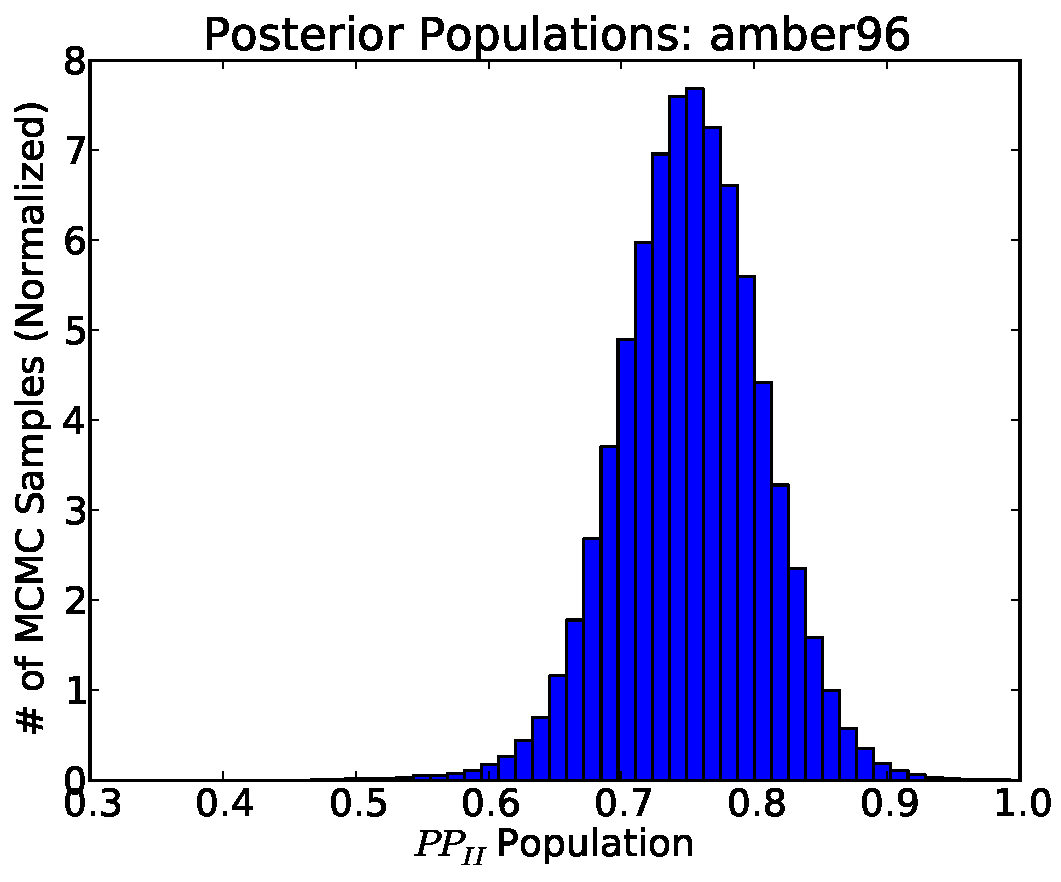
\includegraphics[width=5.25cm]{figures/ALA3_amber96_PPII_MCMC.pdf}
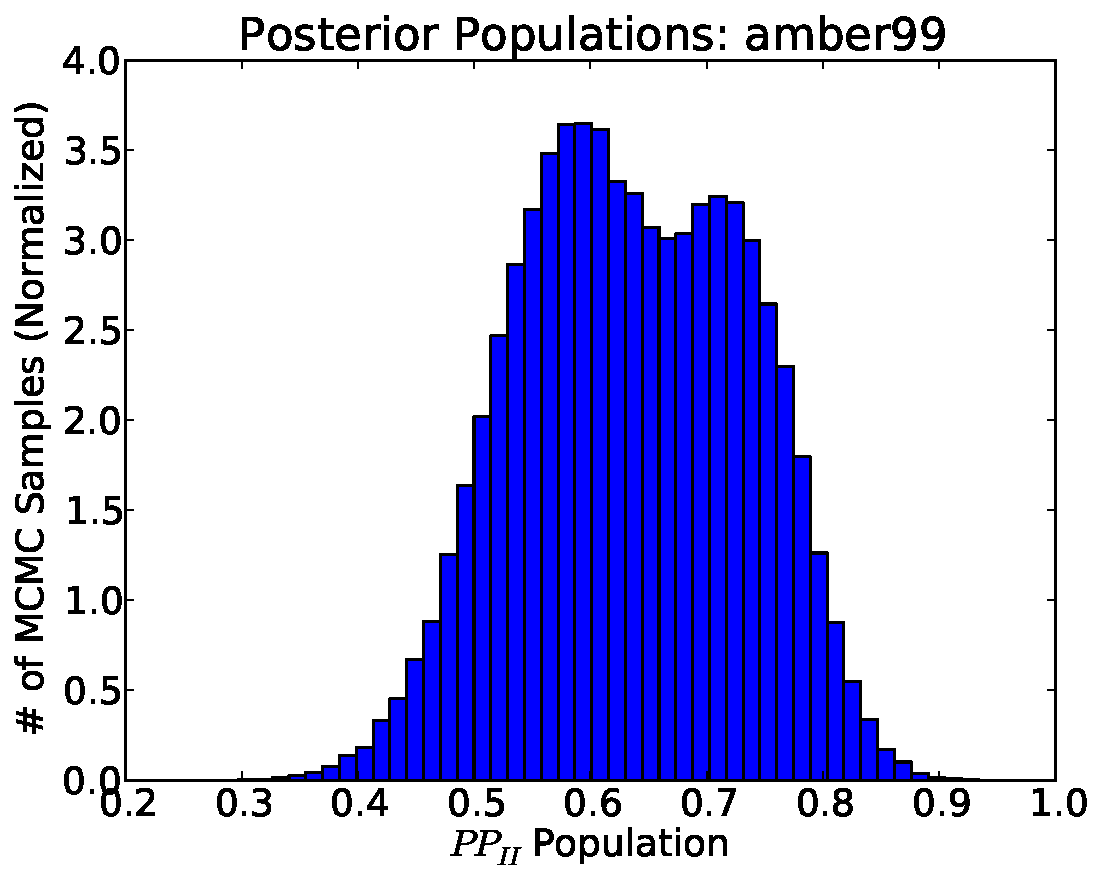
\includegraphics[width=5.25cm]{figures/ALA3_amber99_PPII_MCMC.pdf}

\caption{
Posterior distributions of trialanine $PP_{II}$ populations for amber96 (a) and amber99 (b).  The posterior distribution for amber96 is unimodal, possibly suggesting that a single model is consistent with the simulation and experimental data.  In contrast, the bimodal distribution observed for amber99 implies that two or more models are consistent with the simulation and experimental data.  This highlights the danger in using methods that return a single model, rather the posterior distribution.  
}
\label{figure:ALA3_rama}
\end{figure}

\newpage


\begin{figure}

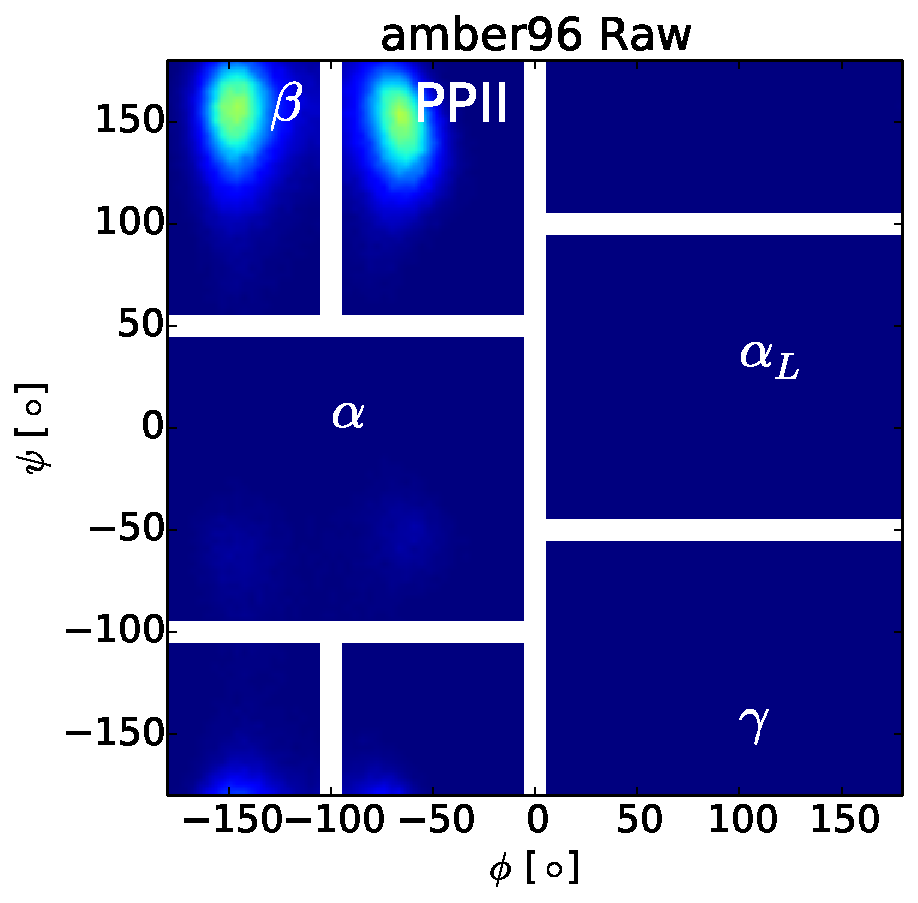
\includegraphics[width=5.25cm]{figures/ALA3_rama_amber96_raw.pdf}
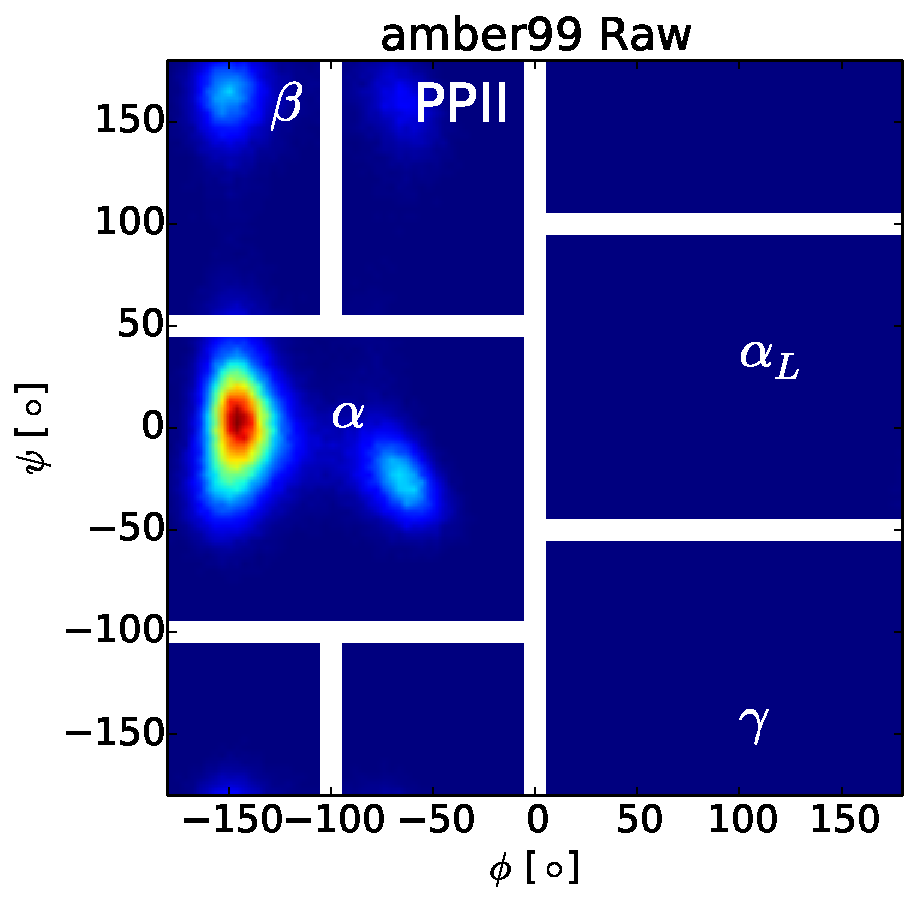
\includegraphics[width=5.25cm]{figures/ALA3_rama_amber99_raw.pdf}
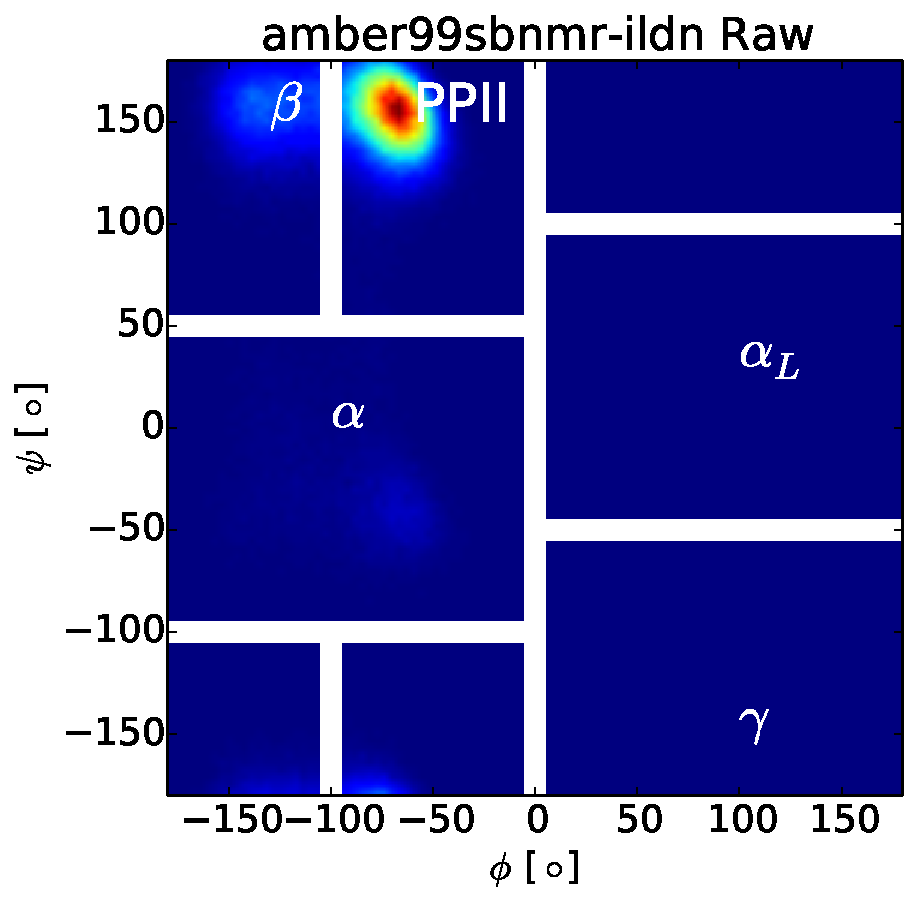
\includegraphics[width=5.25cm]{figures/ALA3_rama_amber99sbnmr-ildn_raw.pdf}

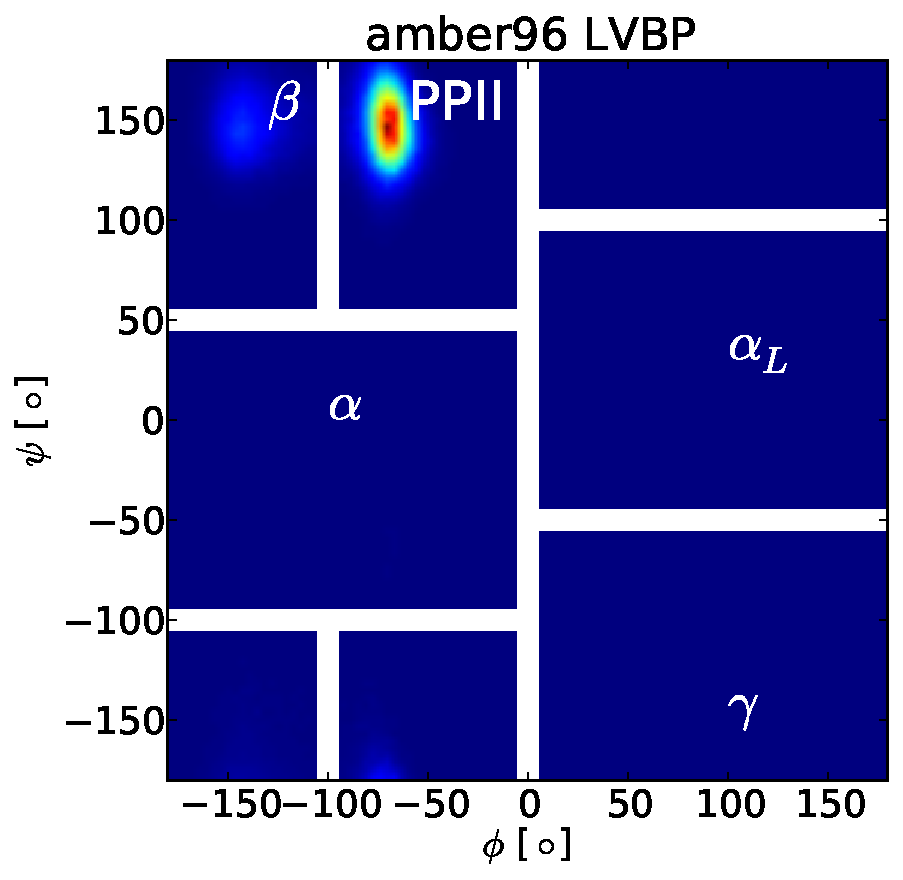
\includegraphics[width=5.25cm]{figures/ALA3_rama_amber96_lvbp.pdf}
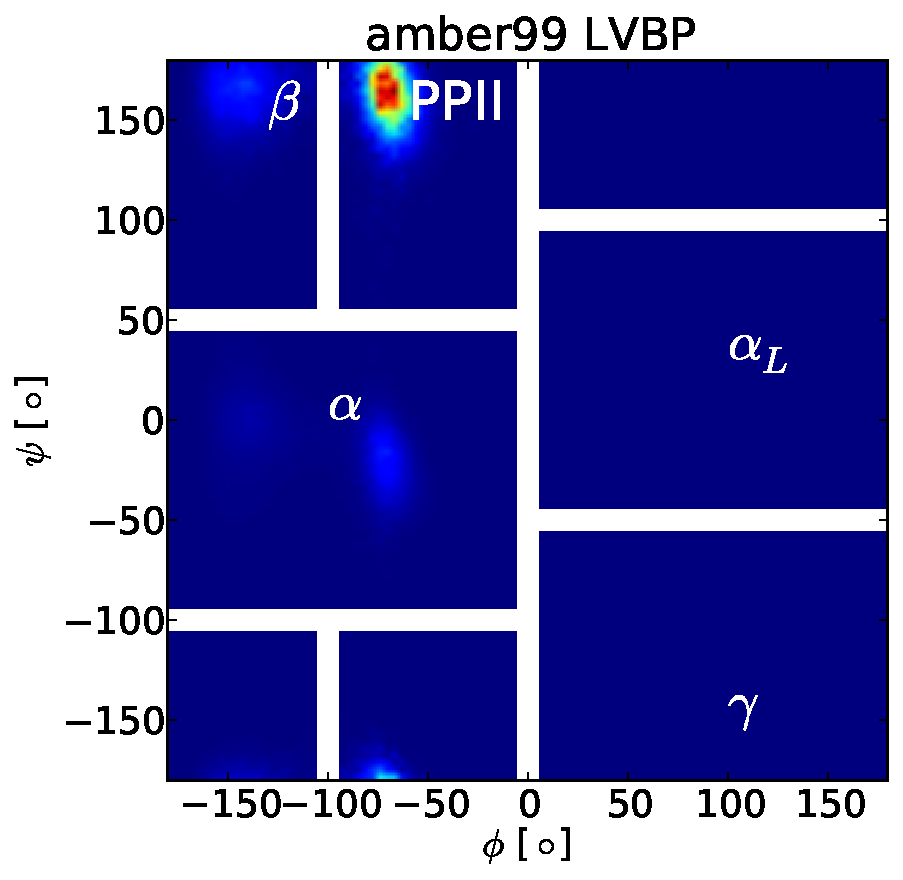
\includegraphics[width=5.25cm]{figures/ALA3_rama_amber99_lvbp.pdf}
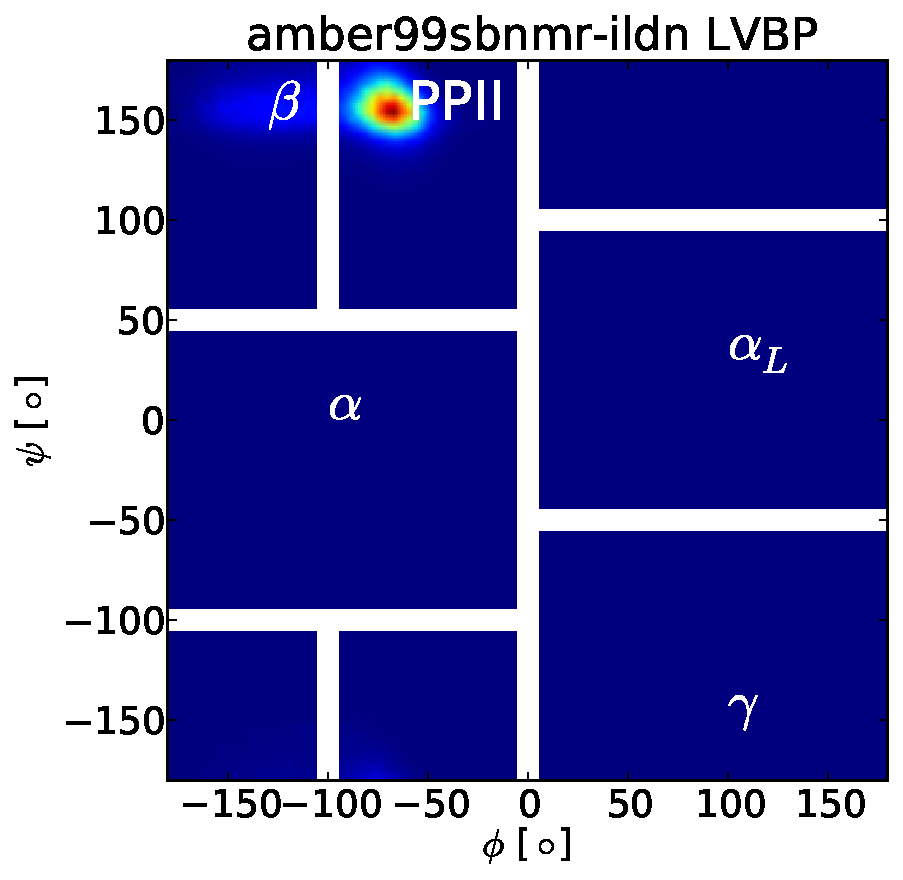
\includegraphics[width=5.25cm]{figures/ALA3_rama_amber99sbnmr-ildn_lvbp.pdf}

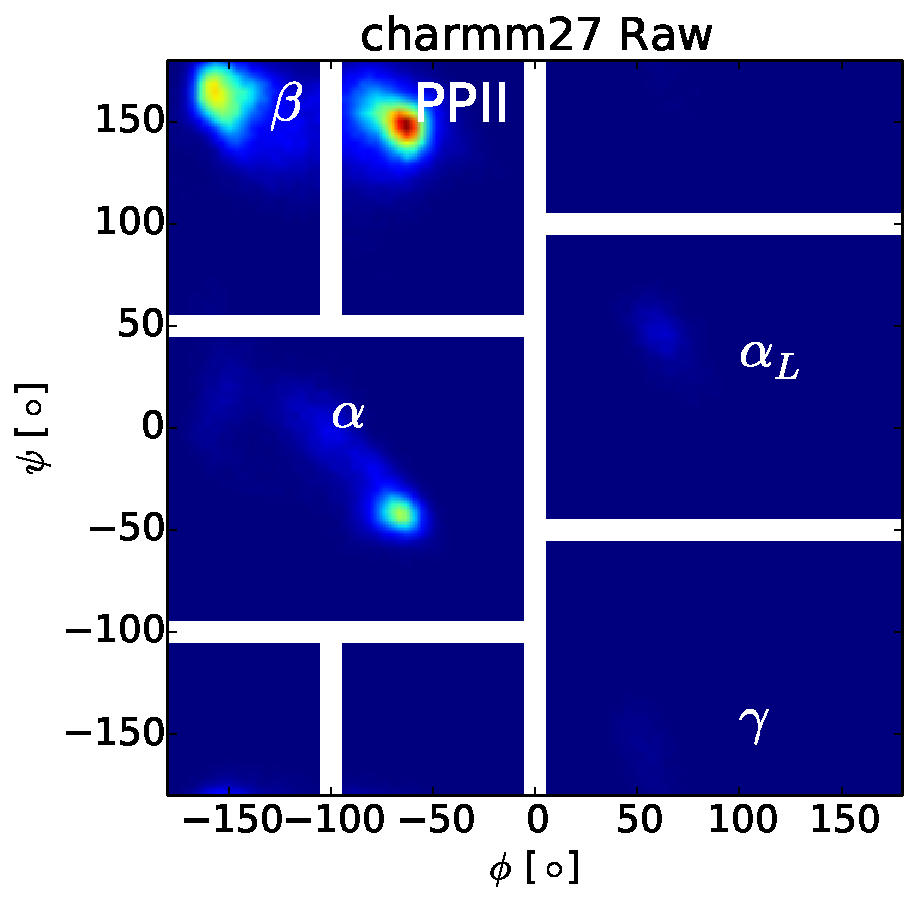
\includegraphics[width=5.25cm]{figures/ALA3_rama_charmm27_raw.pdf}
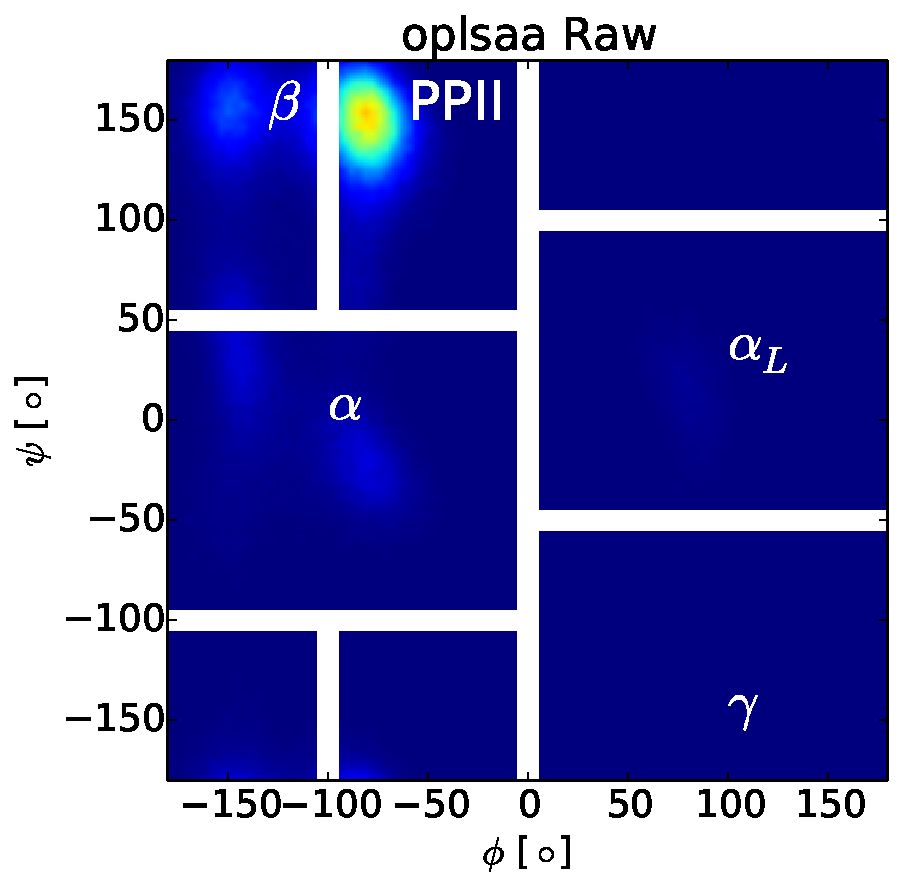
\includegraphics[width=5.25cm]{figures/ALA3_rama_oplsaa_raw.pdf}

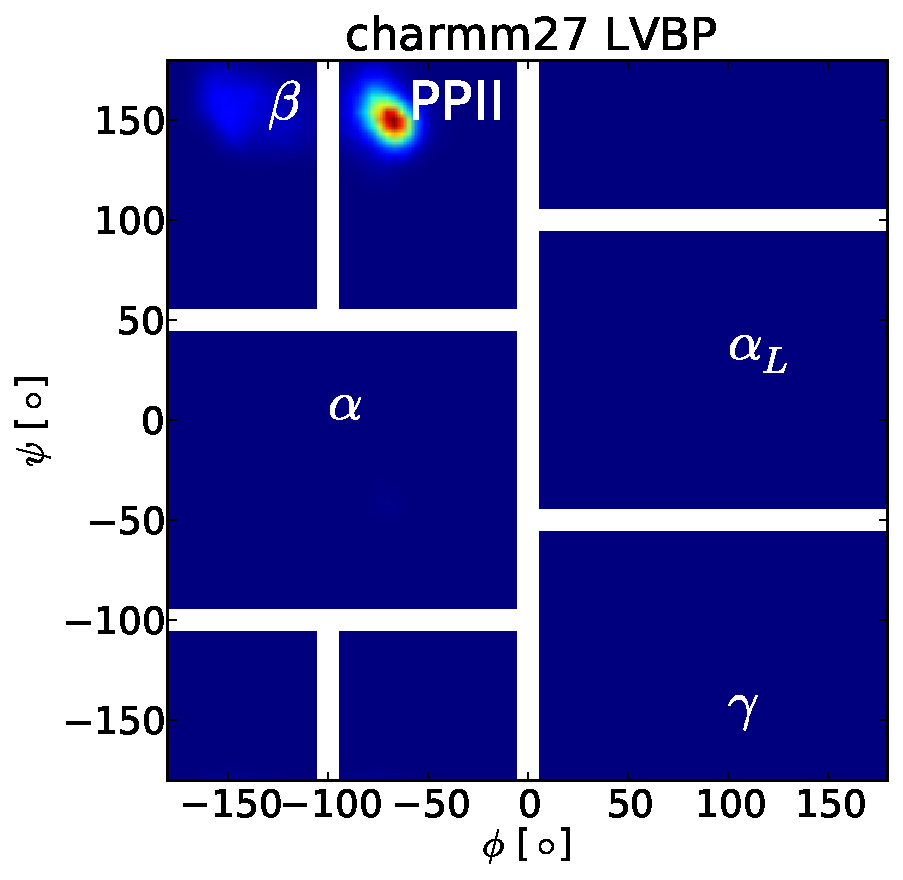
\includegraphics[width=5.25cm]{figures/ALA3_rama_charmm27_lvbp.pdf}
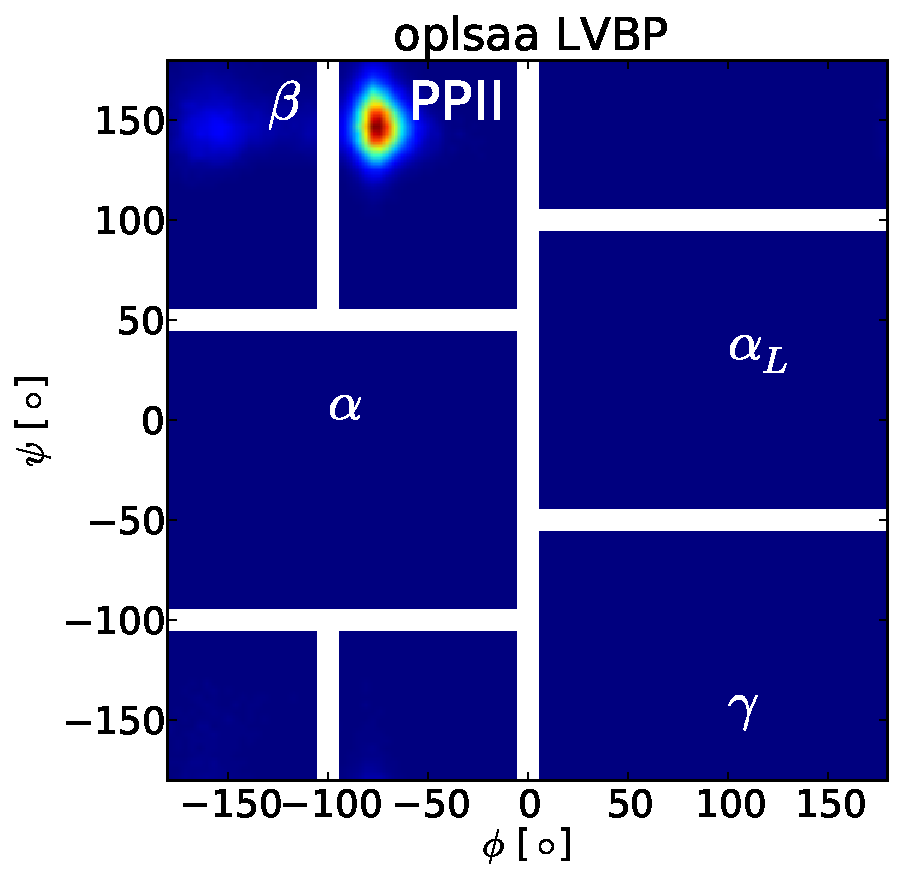
\includegraphics[width=5.25cm]{figures/ALA3_rama_oplsaa_lvbp.pdf}

\caption{
Ramachandran plots (e.g. population densities) of trialanine in five force fields.  Both raw MD results and LVBP ensembles are shown.  State boundaries are plotted as described in ref \cite{Jha2005}.  
}
\label{figure:ALA3_rama}
\end{figure}

\newpage

\begin{figure}
\subfigure[]{
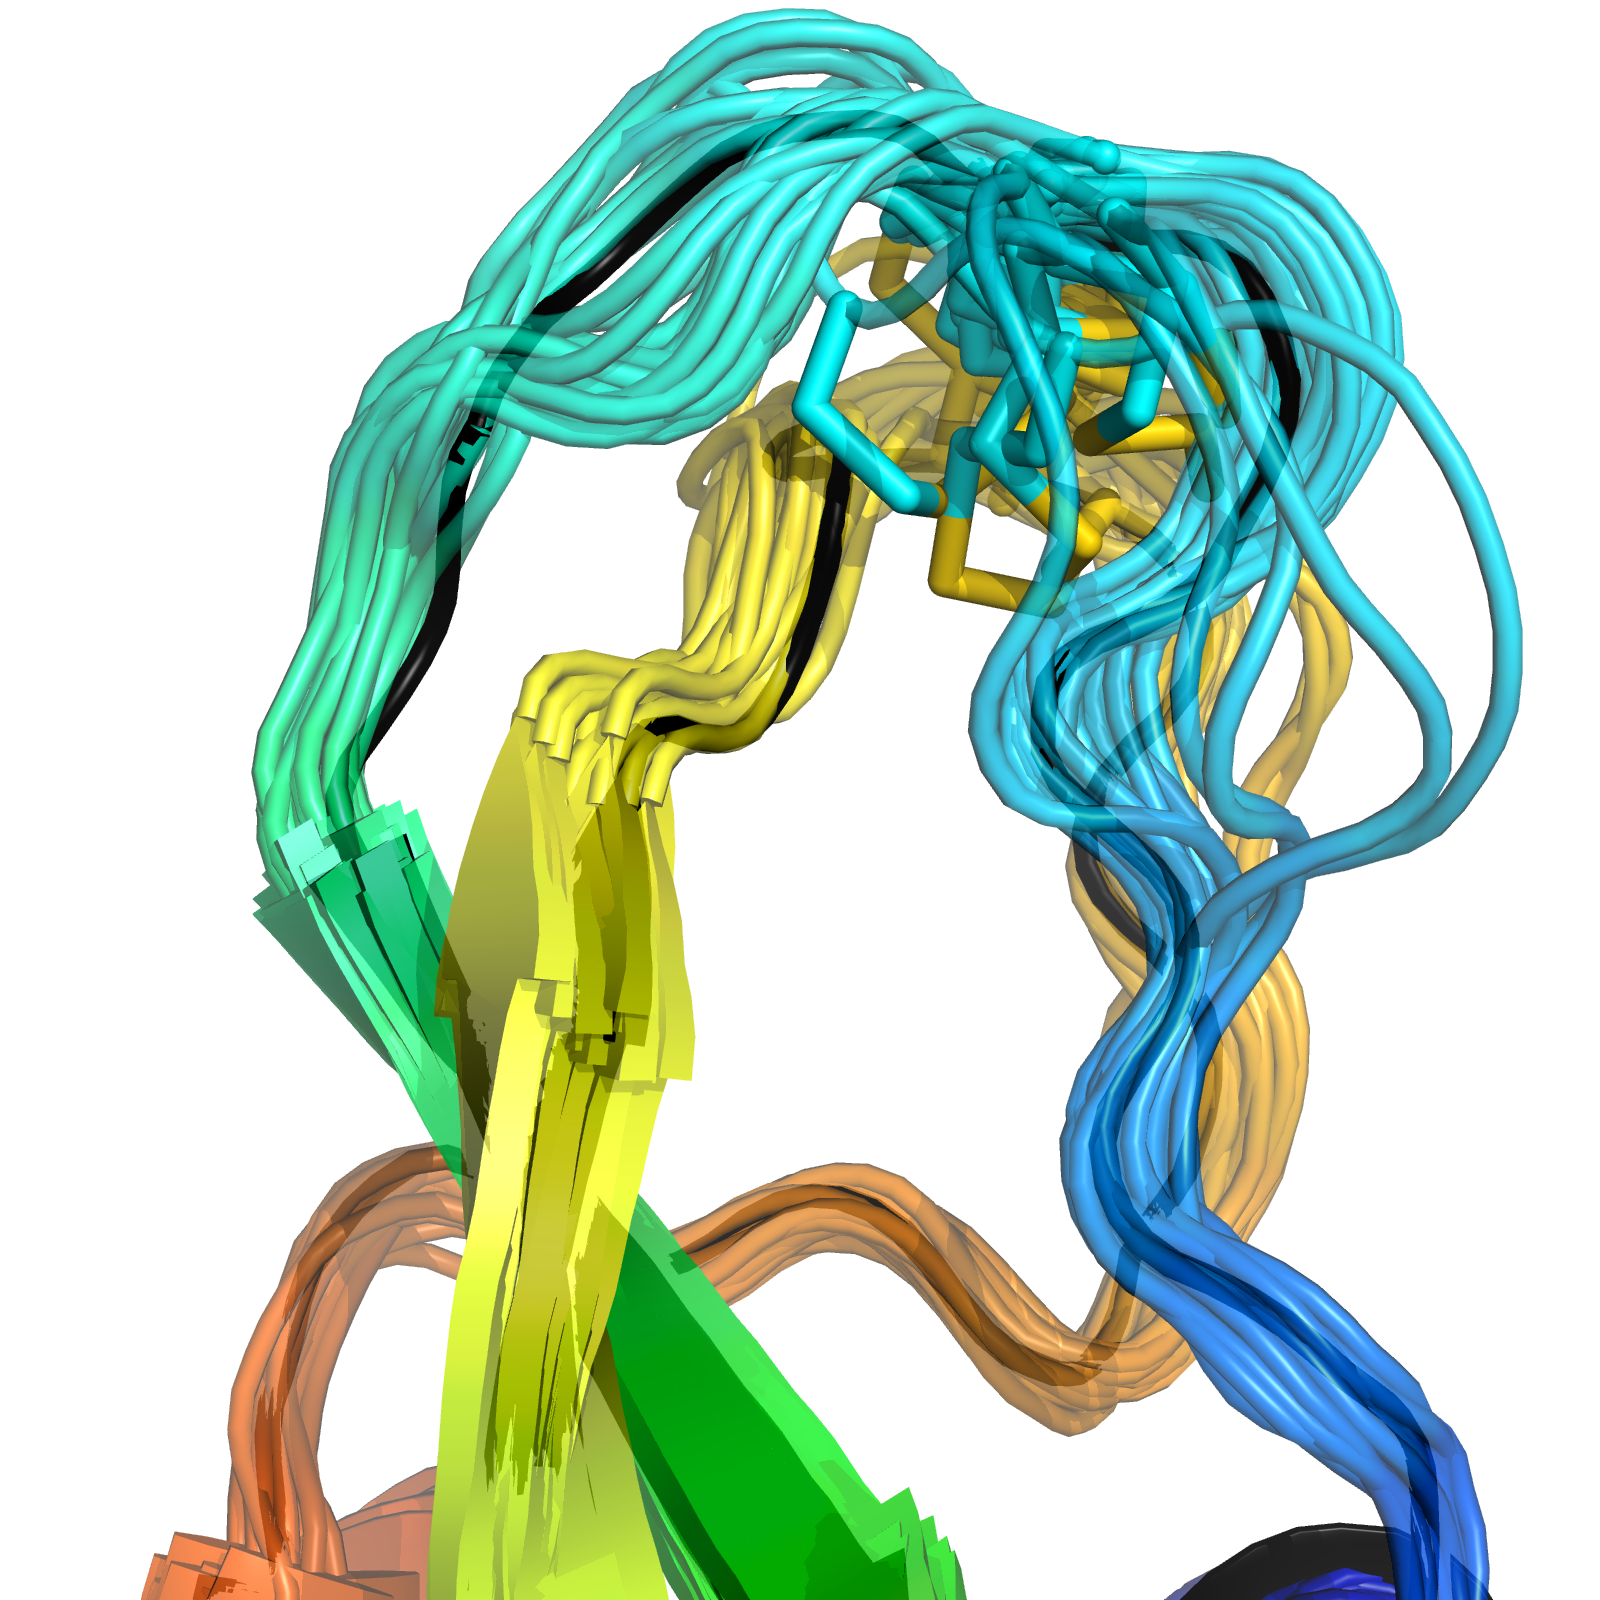
\includegraphics[width=10cm]{figures/bpti_raw.png}
}
\subfigure[]{
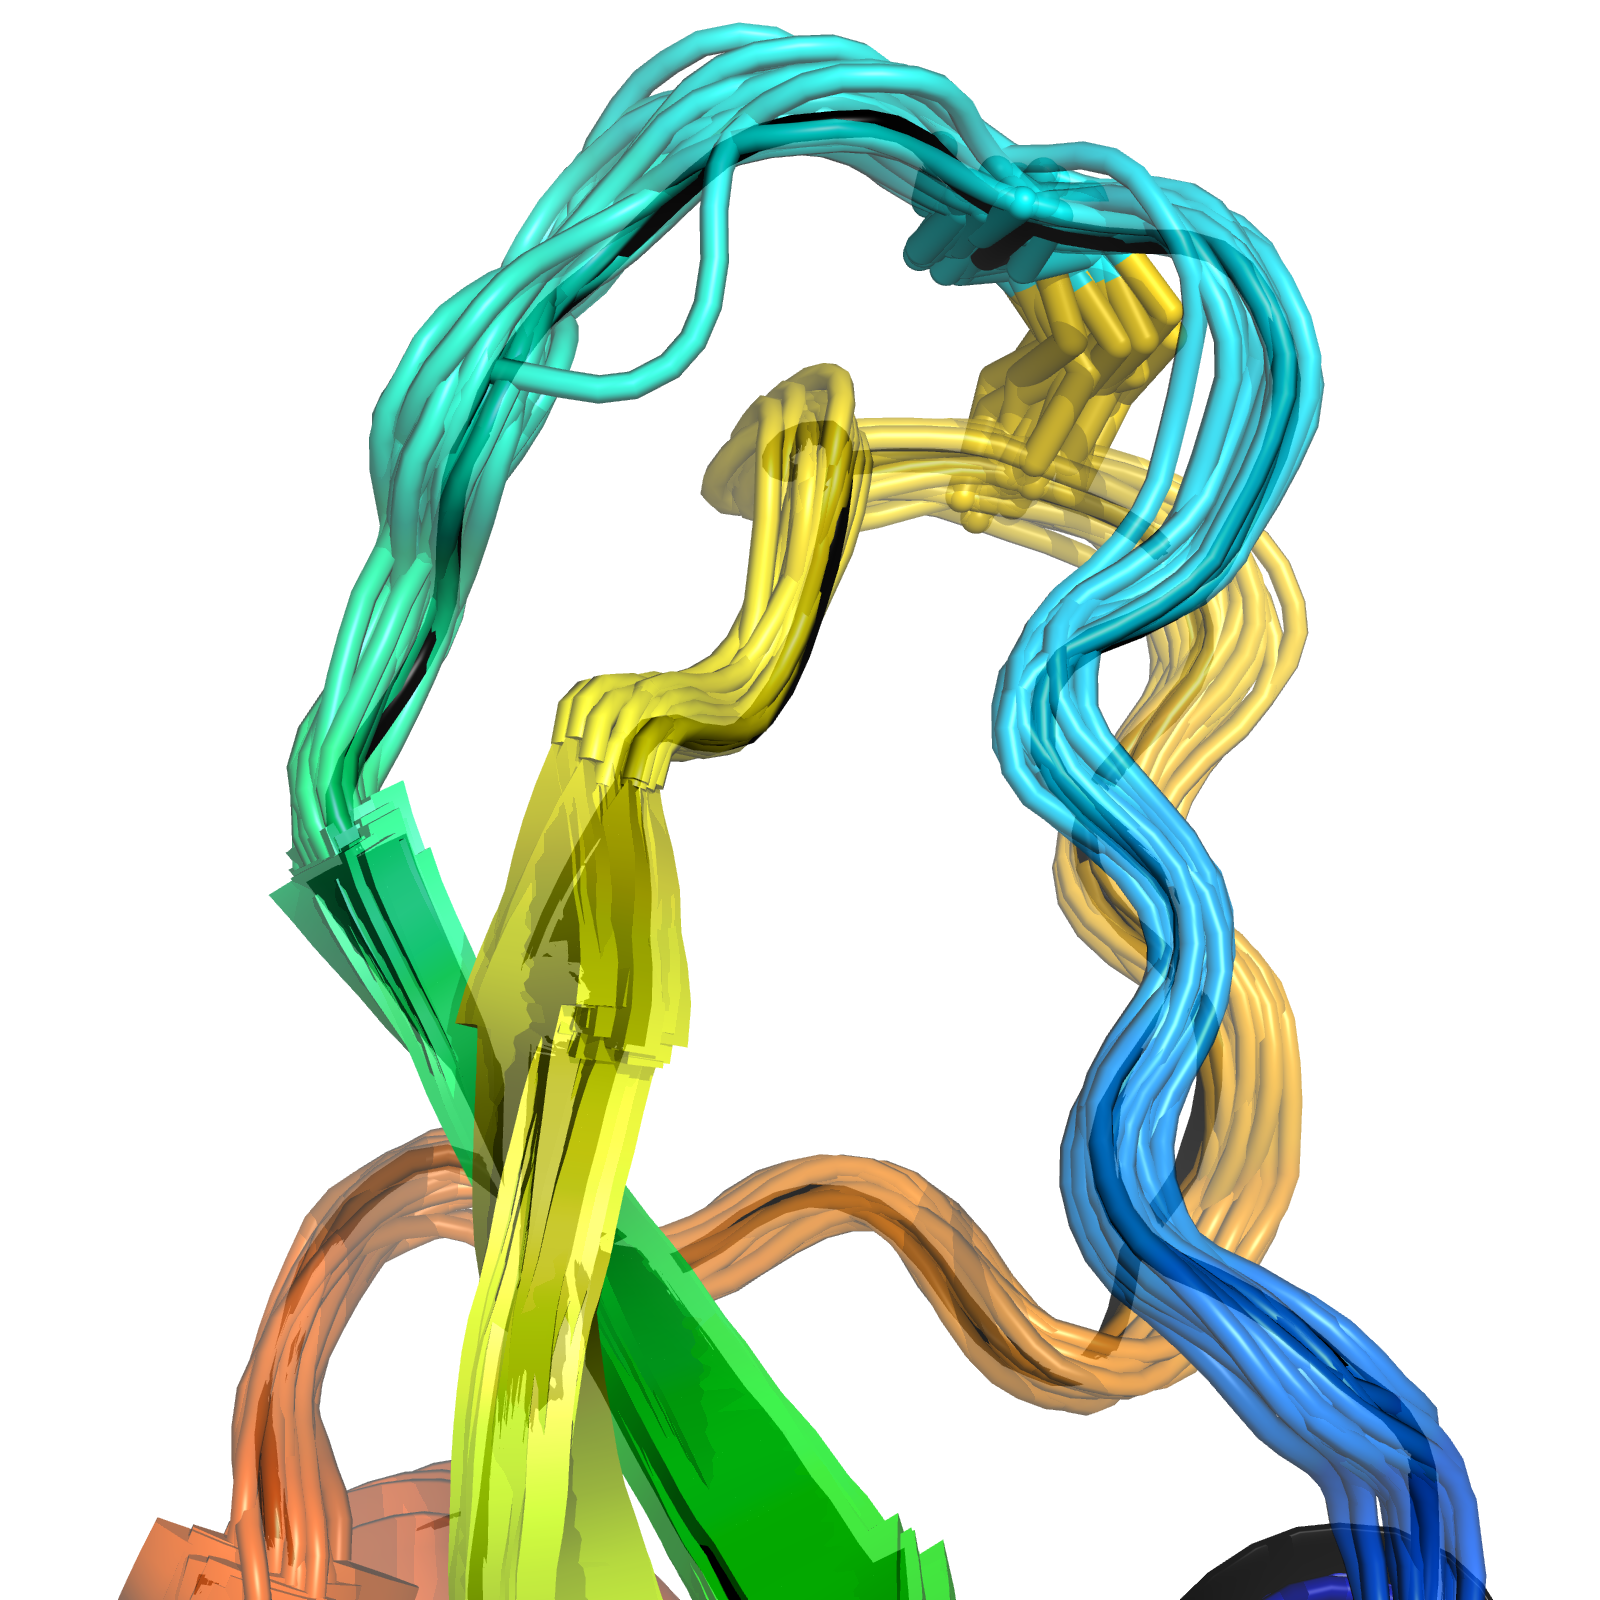
\includegraphics[width=10cm]{figures/bpti_lvbp.png}
}

\caption{
Thirty random snapshots from the MD (a) and LVBP (b) models.  The crystal structure 1BPI \cite{parkin1996structure} is shown in black.  The trypsin binding loop is located at the top, with residues C14 and C38 shown as sticks.  
}
\label{figure:PDB_BPTI}
\end{figure}


\newpage


\begin{figure}
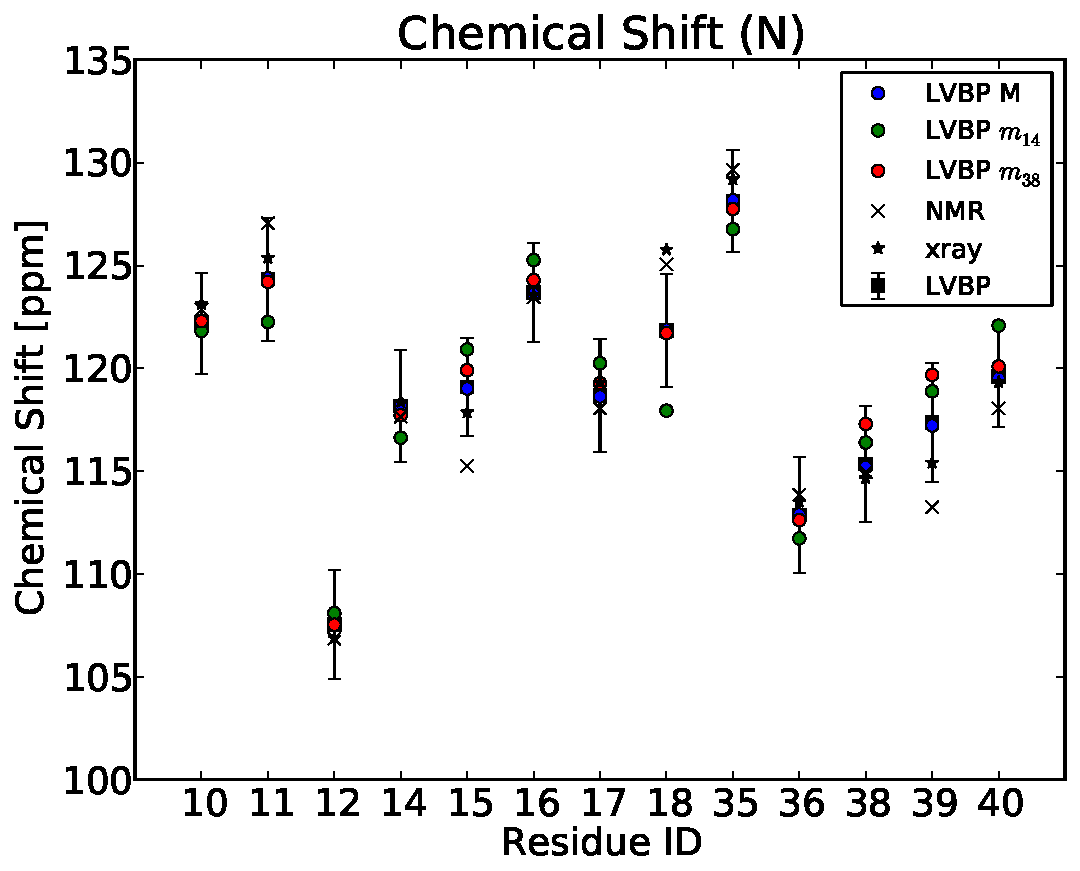
\includegraphics[width=8cm]{figures/BPTI_shifts_N.pdf}
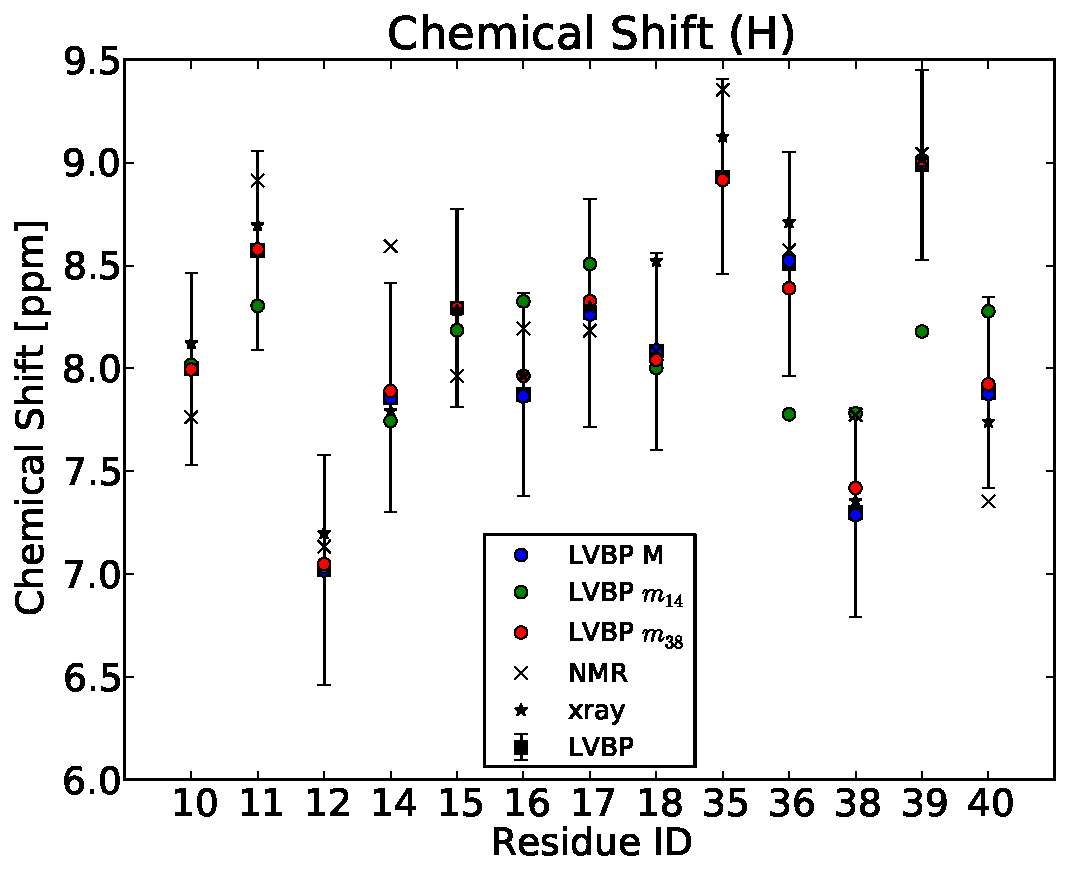
\includegraphics[width=8cm]{figures/BPTI_shifts_H.pdf}

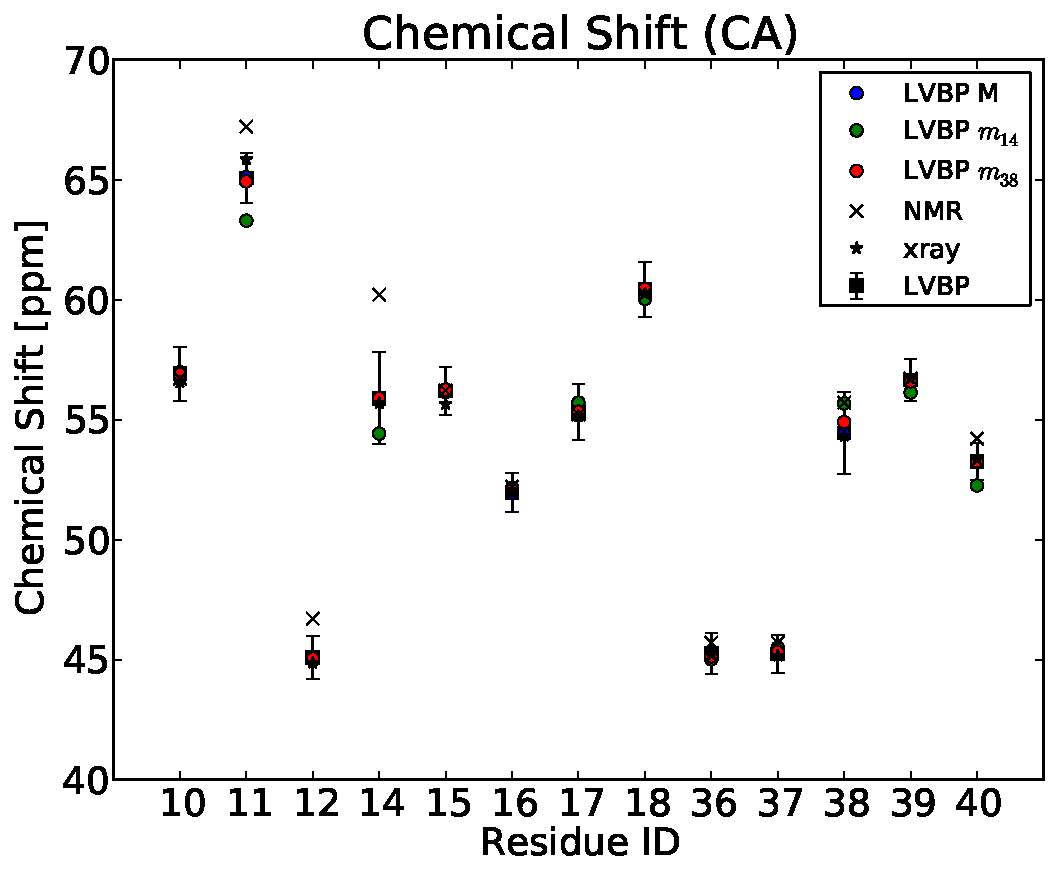
\includegraphics[width=8cm]{figures/BPTI_shifts_CA.pdf}
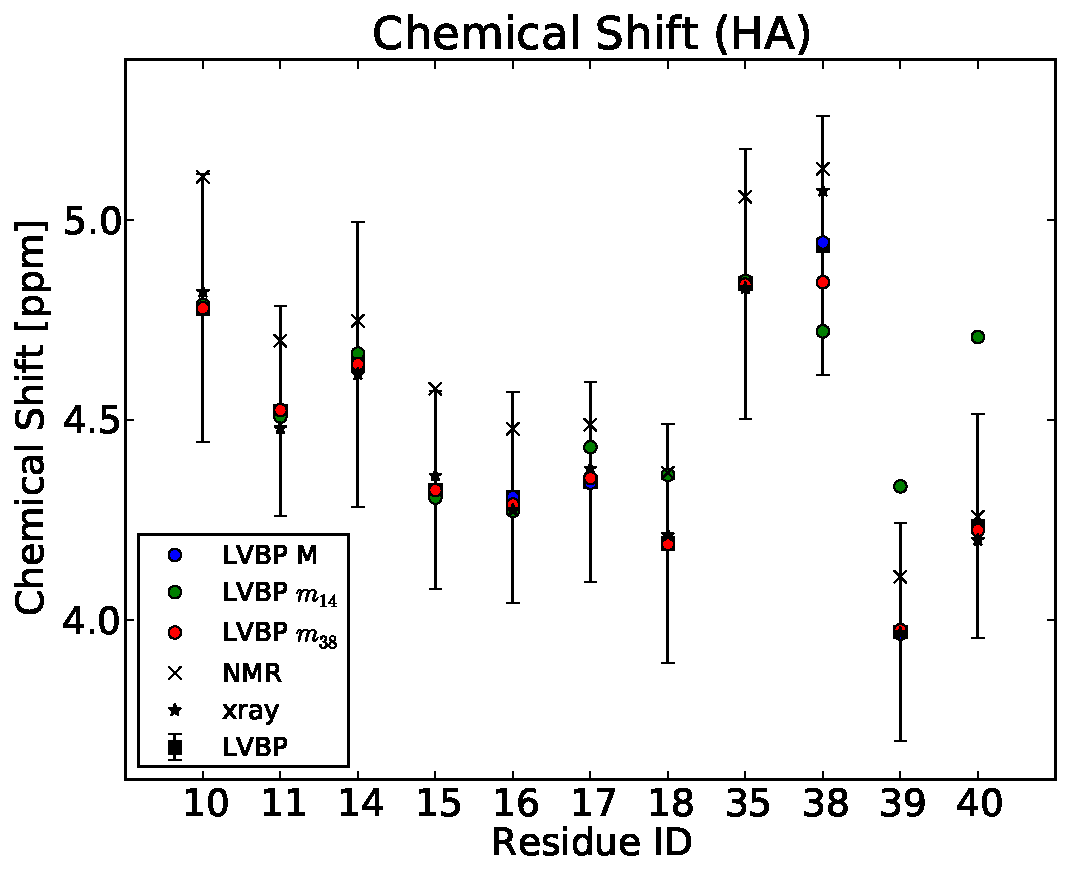
\includegraphics[width=8cm]{figures/BPTI_shifts_HA.pdf}
\caption{
Predicted chemical shifts of BPTI.  The LVBP predictions are shown as black squares with error bars given by the chemical shift prediction uncertainty.  The LVBP-average chemical shift of conformational substates are shown as colored circles.  The experimentally-measured chemical shifts are shown as black Xs.  The X-ray predicted chemical shifts are given as black stars.  
}
\label{figure:BPTI_Shifts}
\end{figure}

\newpage

\begin{figure}
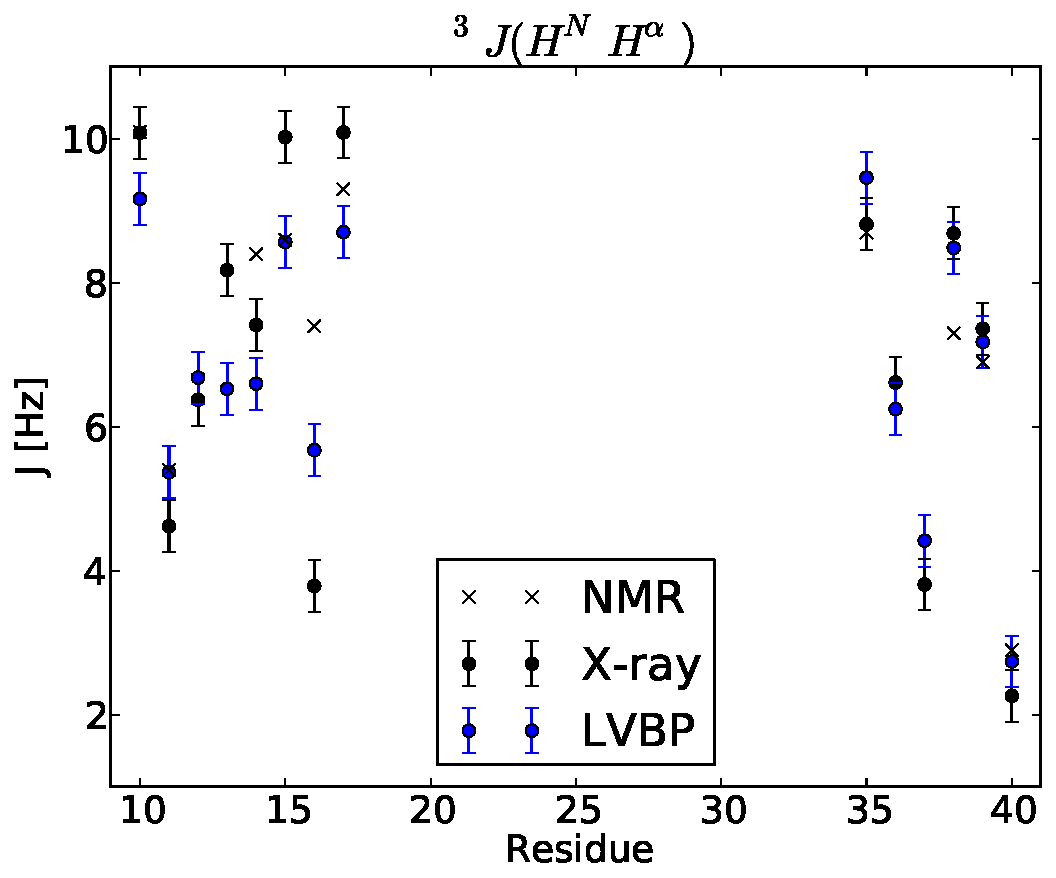
\includegraphics[width=8cm]{figures/BPTI_couplings_J3_HN_HA.pdf}
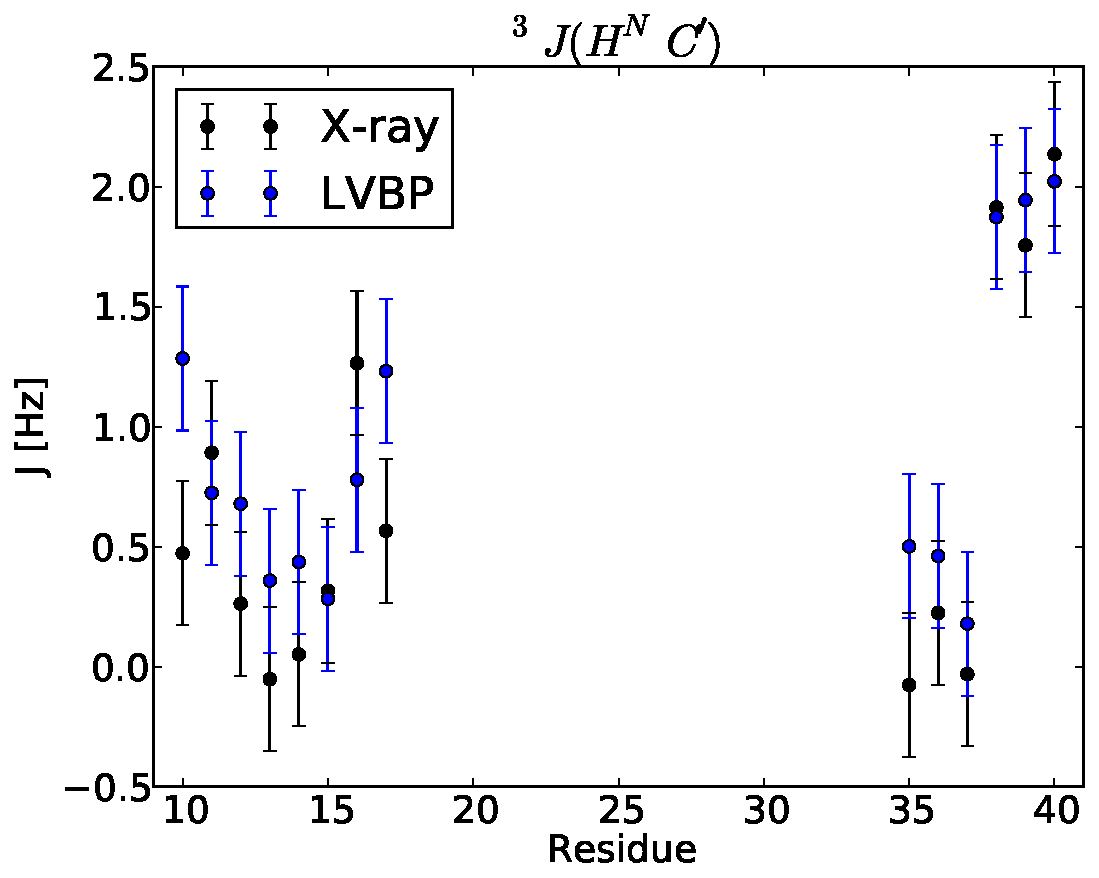
\includegraphics[width=8cm]{figures/BPTI_couplings_J3_HN_Cprime.pdf}

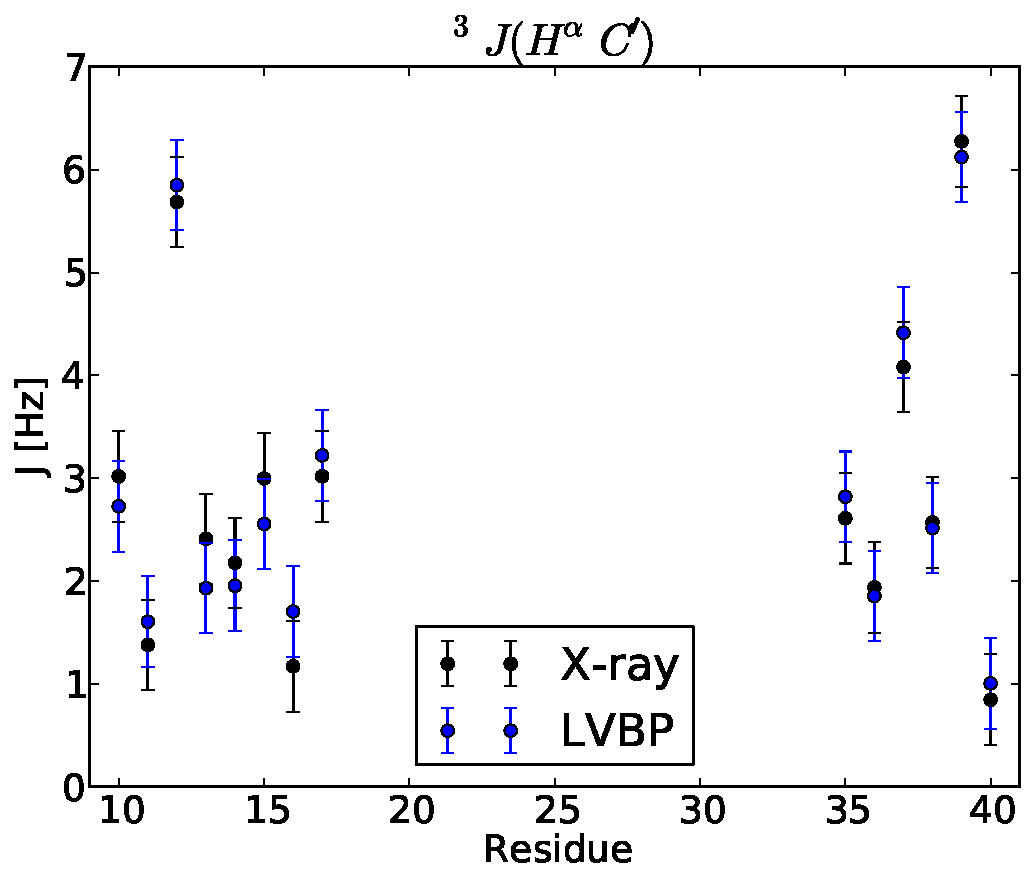
\includegraphics[width=8cm]{figures/BPTI_couplings_J3_HA_Cprime.pdf}
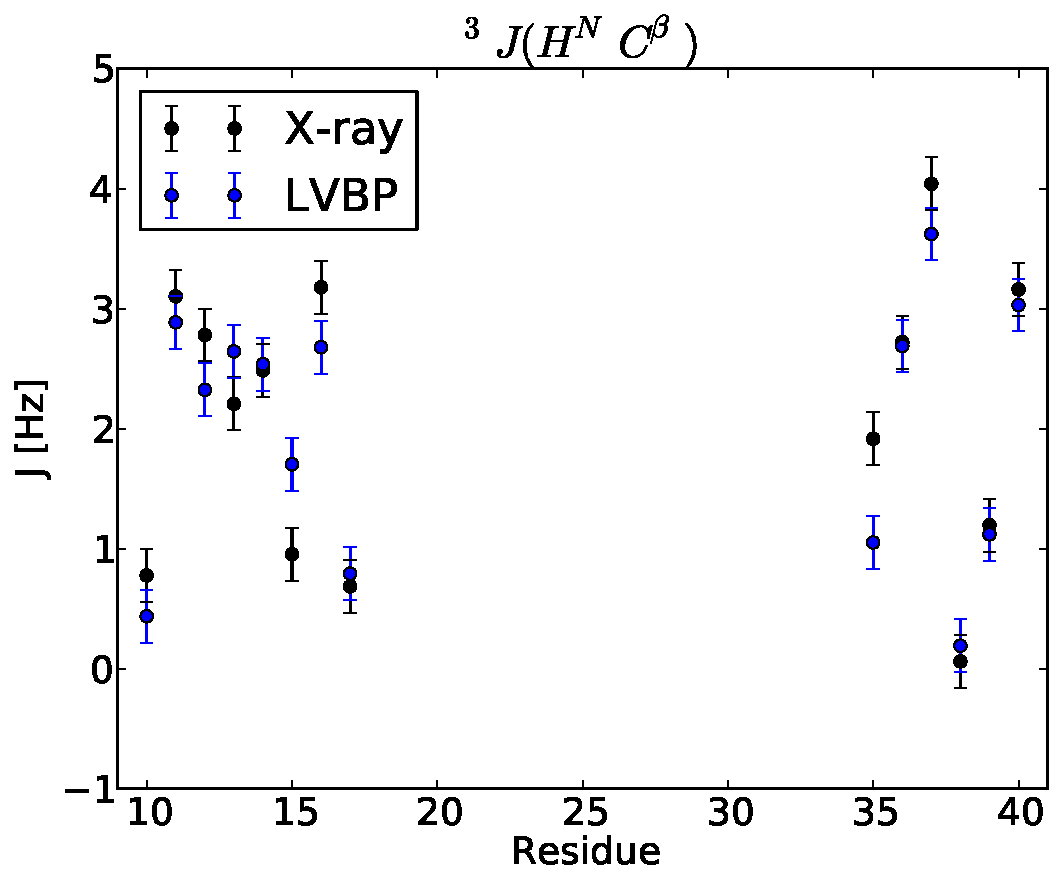
\includegraphics[width=8cm]{figures/BPTI_couplings_J3_HN_CB.pdf}

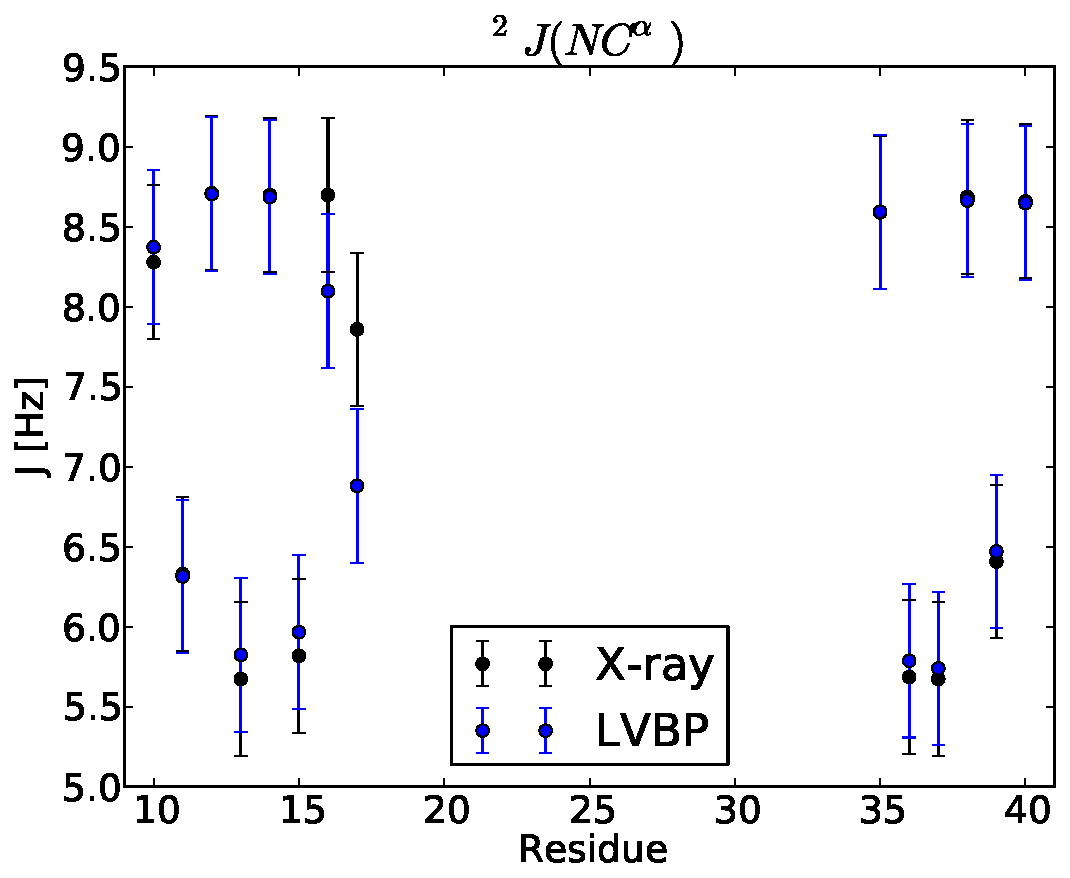
\includegraphics[width=8cm]{figures/BPTI_couplings_J2_N_CA.pdf}
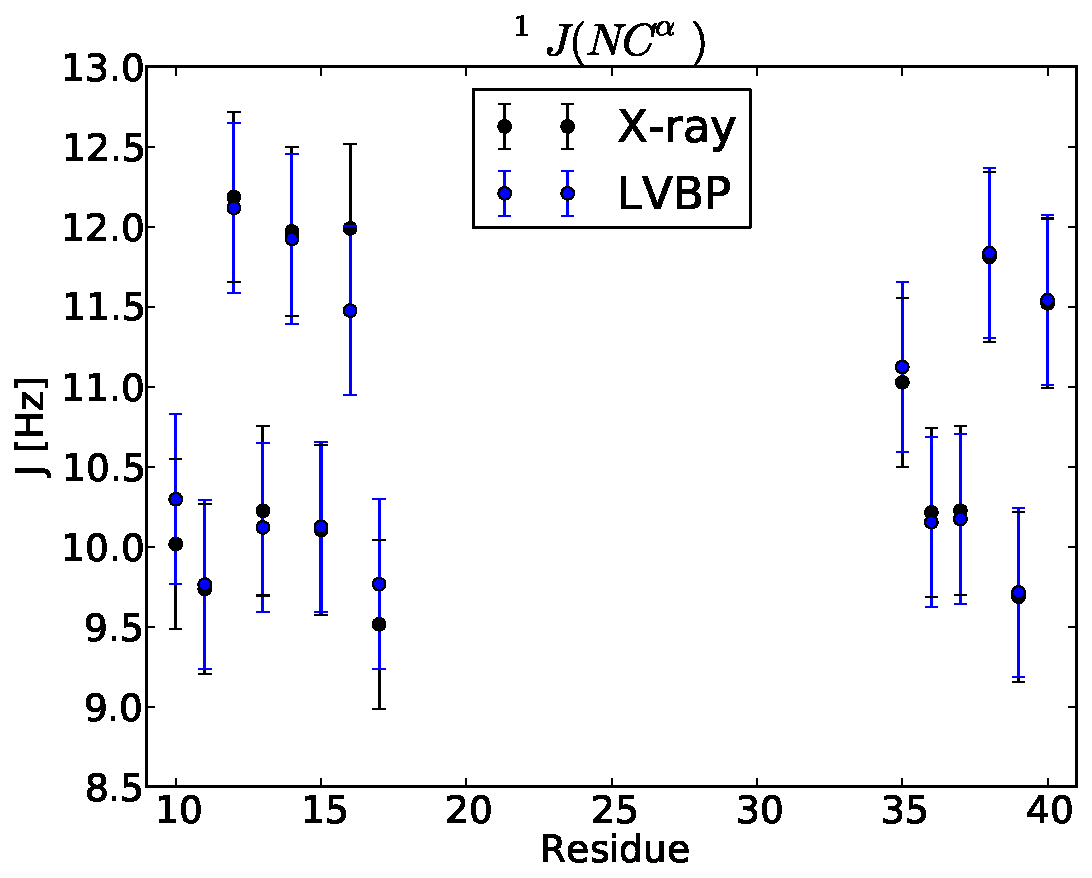
\includegraphics[width=8cm]{figures/BPTI_couplings_J1_N_CA.pdf}
\caption{
Predicted scalar couplings of BPTI.  Predictions are made using both the LVBP and X-ray models.  The few available measurements (for  $^3J(H^N H^\alpha)$) are shown as Xs.  
}
\label{figure:bpti_couplings}
\end{figure}

\newpage


\begin{figure}
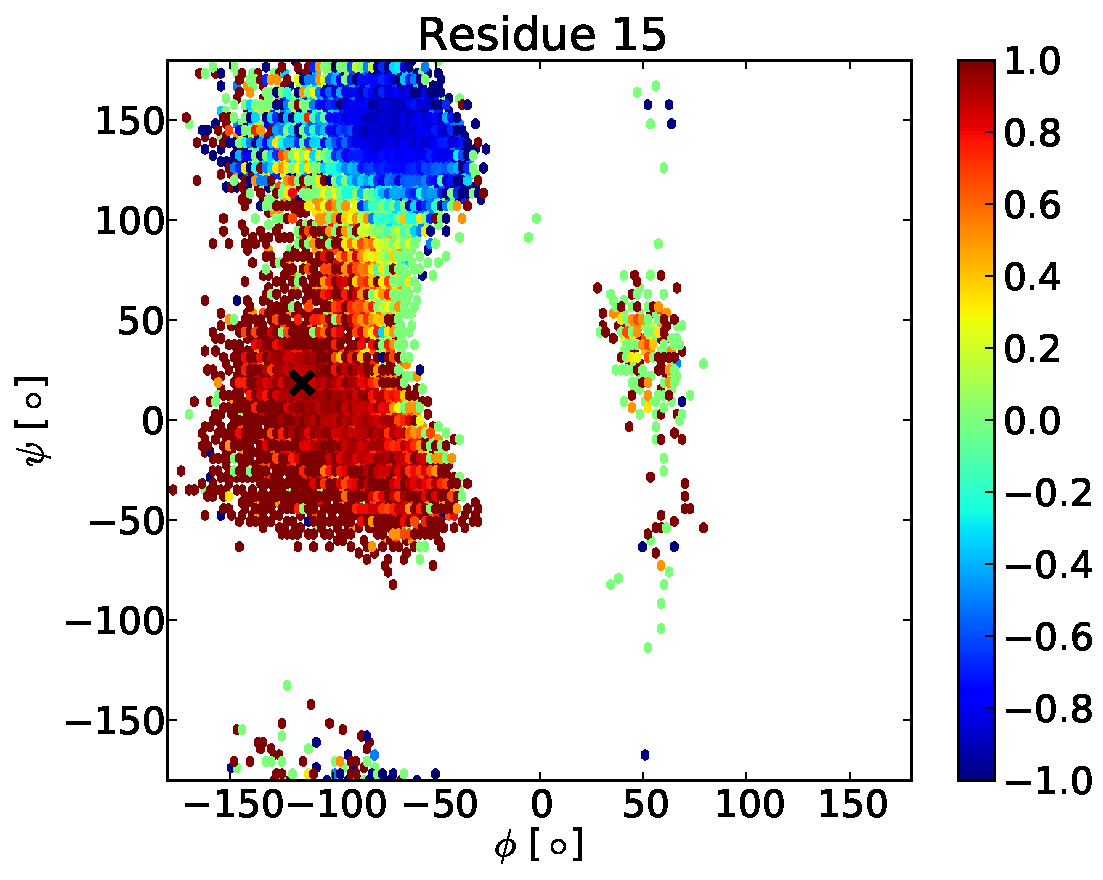
\includegraphics[width=8cm]{figures/BPTI_backbone_torsion_states_15.pdf}
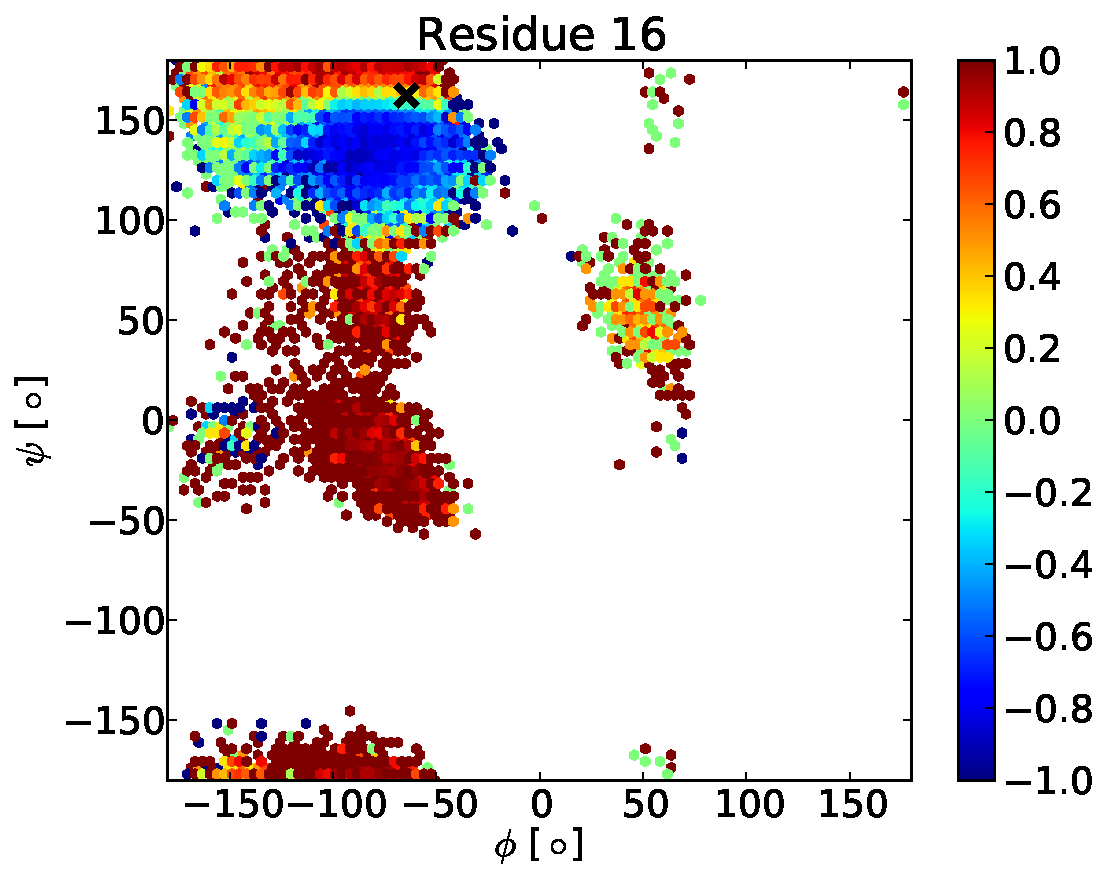
\includegraphics[width=8cm]{figures/BPTI_backbone_torsion_states_16.pdf}
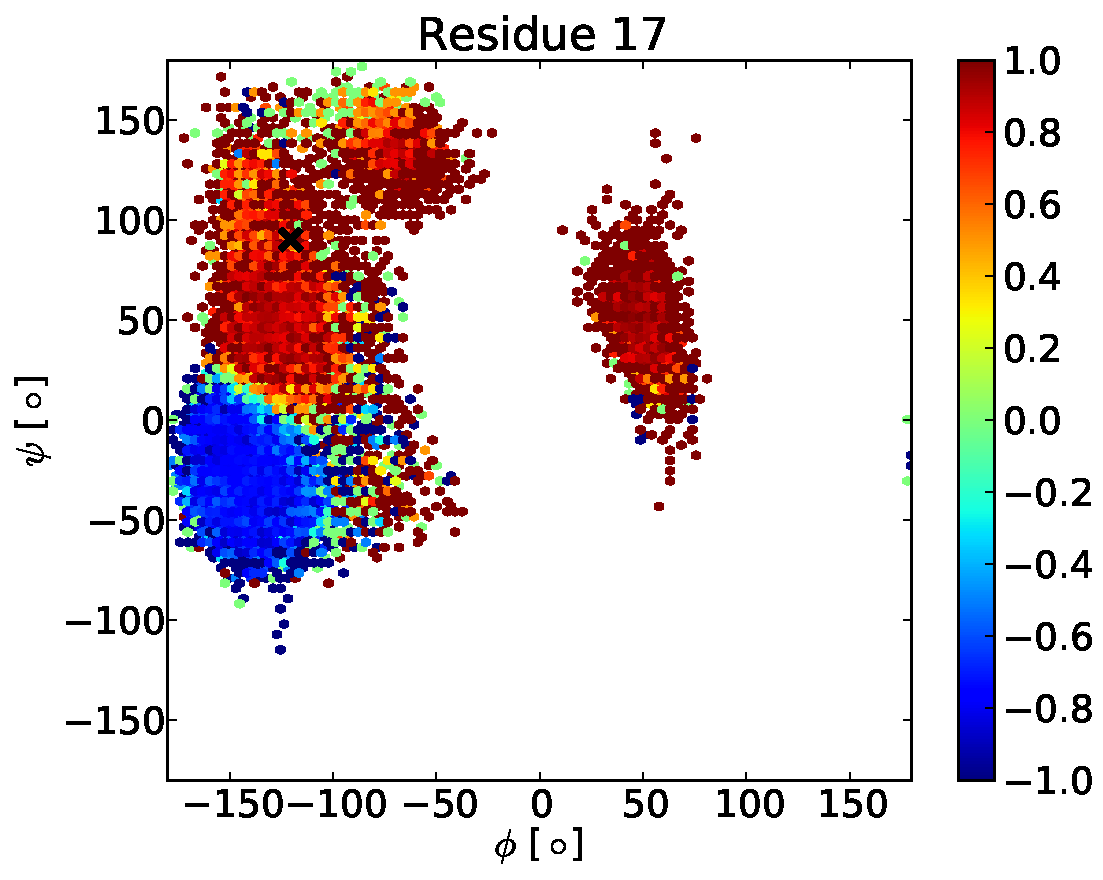
\includegraphics[width=8cm]{figures/BPTI_backbone_torsion_states_17.pdf}
\caption{
The $M$ and $m_{14}$ $\chi_1$ torsional states are projected onto backbone torsions in the trypsin specificity site.  Values near 1 indicate regions belonging to the $M$ torsional state, while values near -1 indicate regions belonging to $m_{14}$ torsional state.  Intermediate values indicate regions that are not well-separated by the $M$ and $m_{14}$ conformational states.  We observe that the $\phi$, $\psi$ basins tend to be well-separated by the $M$ and $m_{14}$ $\chi_1$ torsional states.  Thus, the backbone motion in residues 15, 16, and 17 tends to be coupled to the disulfide-bond rotation.  We also plot the crystallographic $\phi$ and $\psi$ angles (X) for reference.  
}
\label{figure:bpti_backbone_states}
\end{figure}

\newpage

\begin{figure}
\subfigure[]{
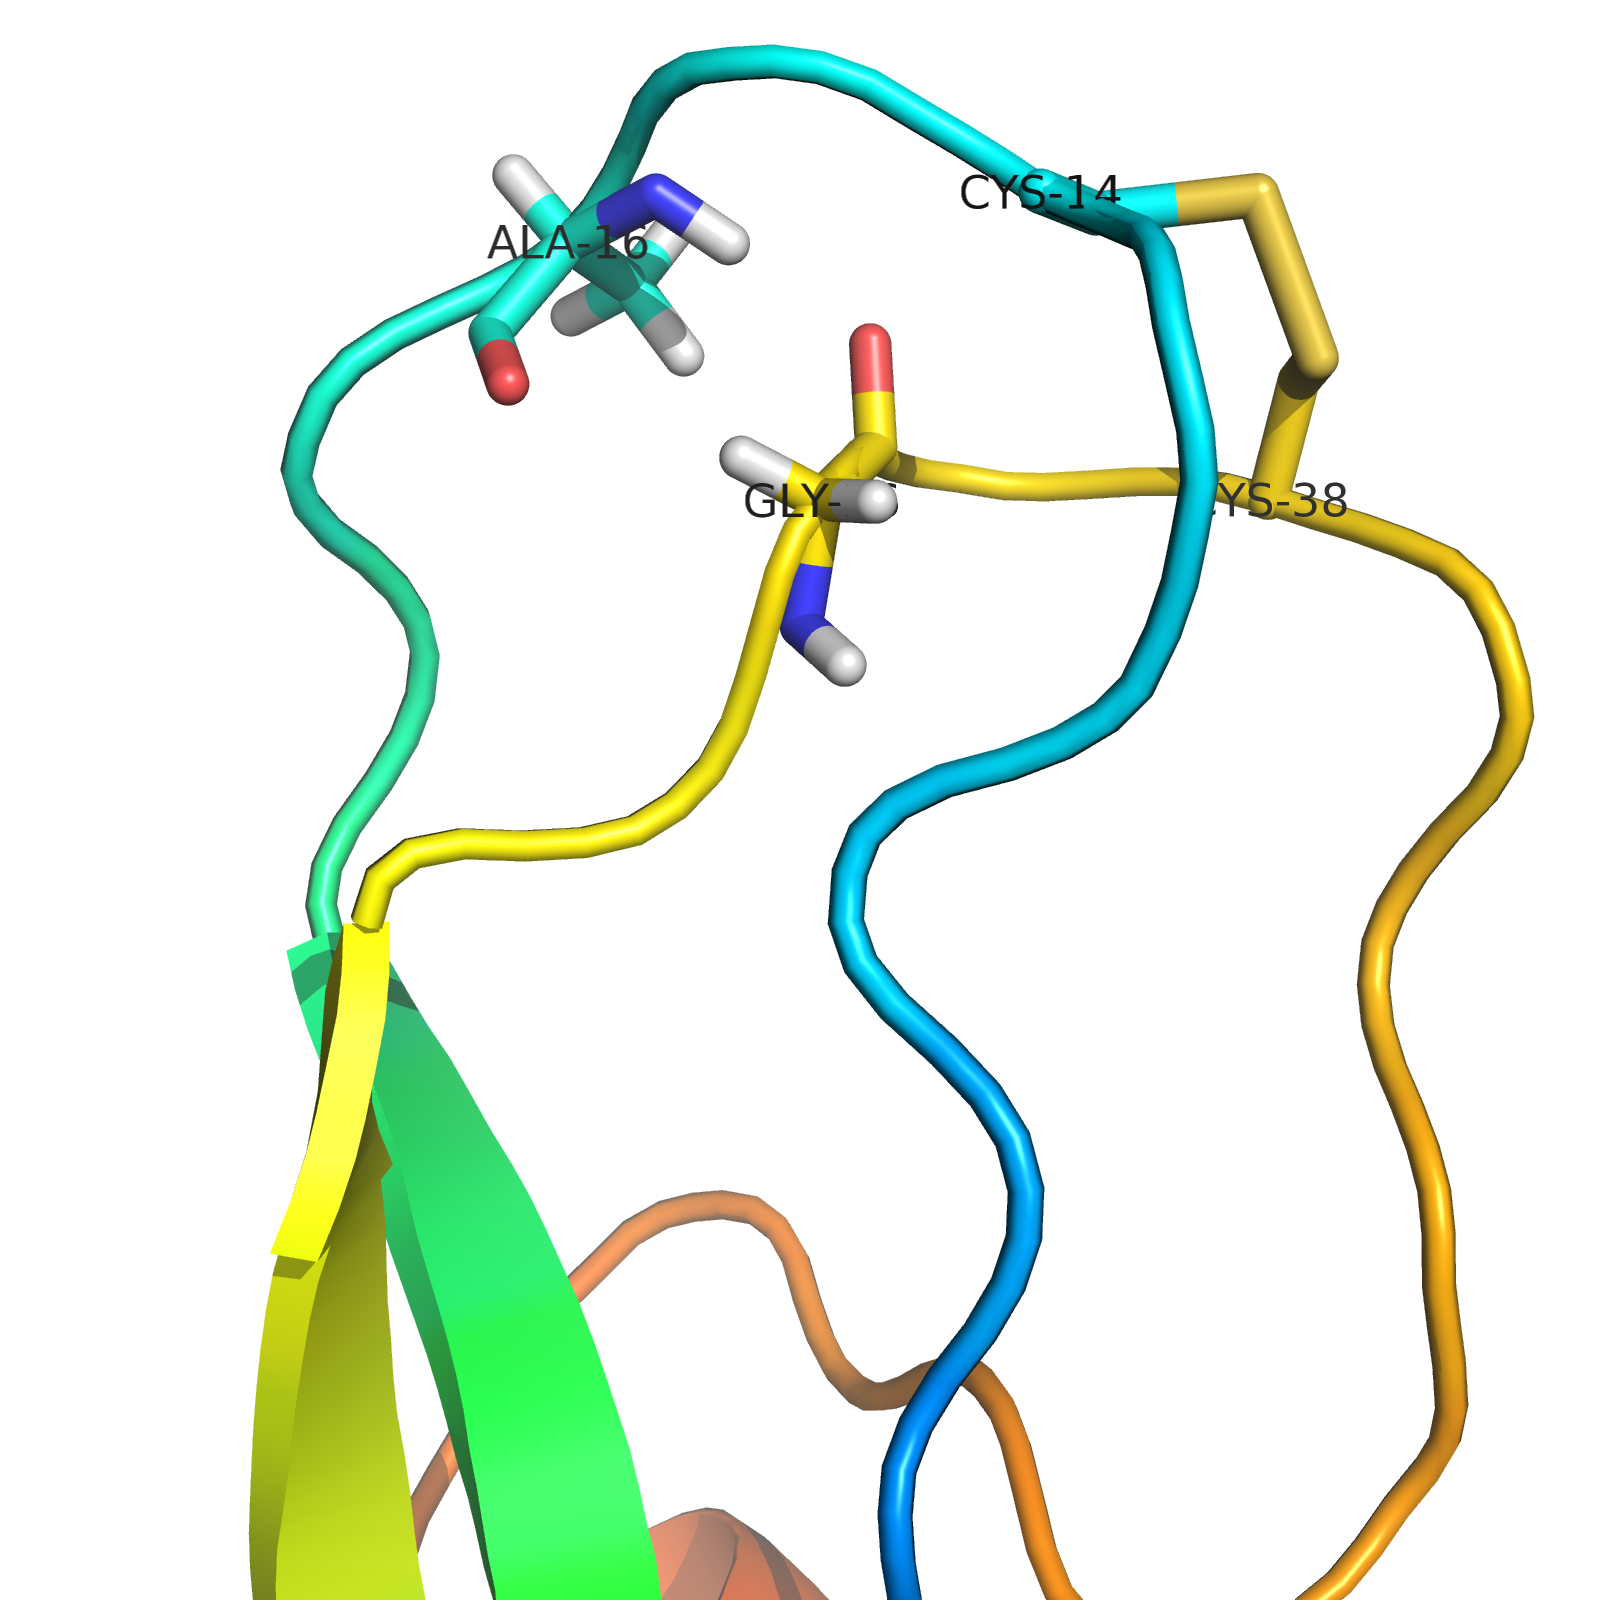
\includegraphics[width=10cm]{figures/bpti_noe_state1.png}
}

\subfigure[]{
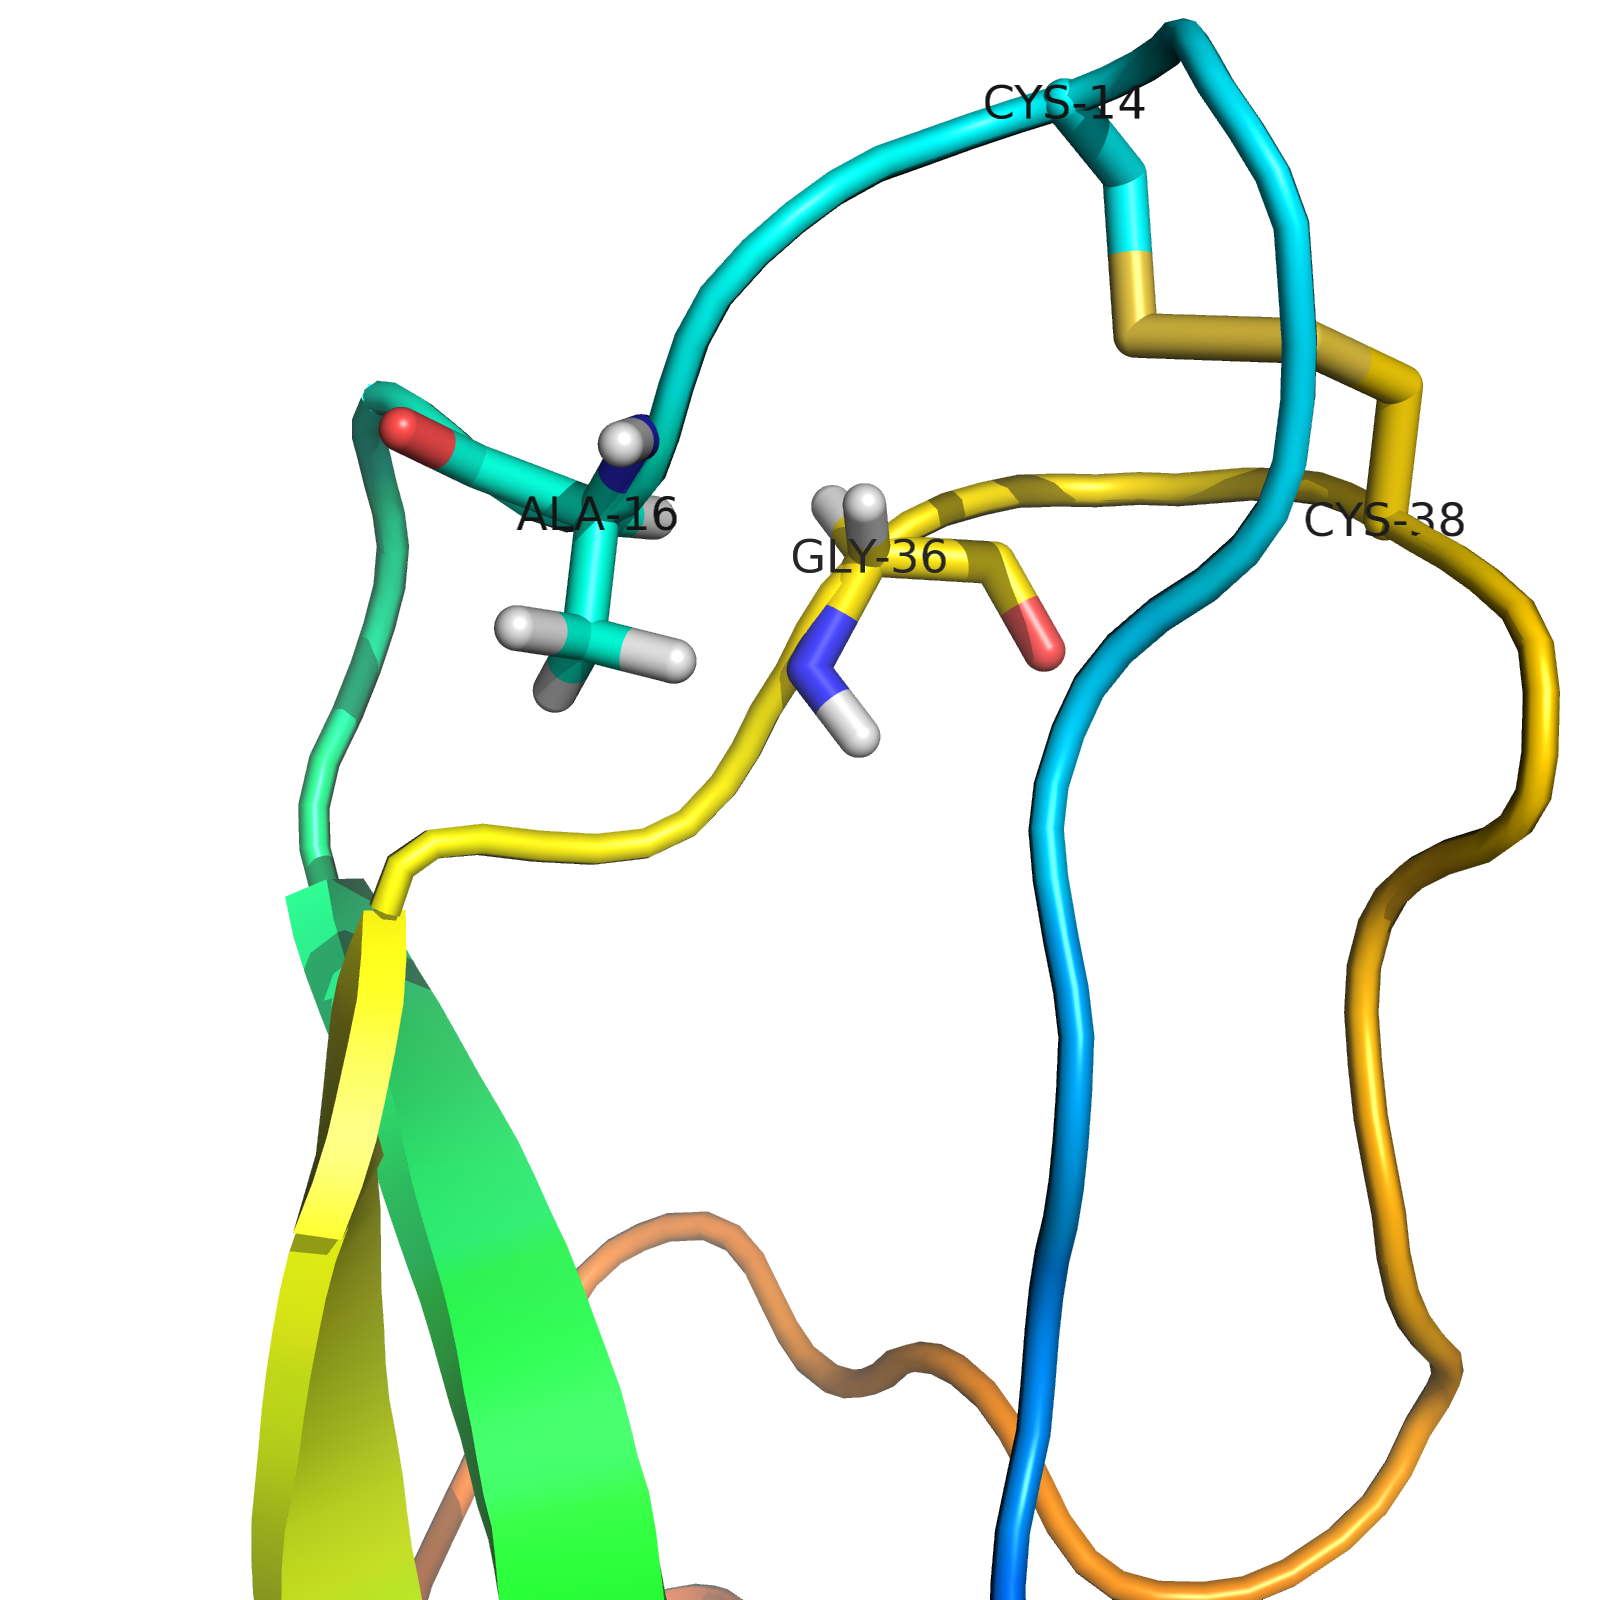
\includegraphics[width=10cm]{figures/bpti_noe_state2.png}
}
\caption{
Non-native tertiary contact present in $m_{14}$, but not in $M$.  (a).  State $M$.  (b).  State $m_{14}$
}
\label{figure:PDB_contact}
\end{figure}

\clearpage

\bibliography{supporting_information}

\end{document}
